% !TEX program = xelatex
% Diplomski rad - LaTeX izvor
% Kompajlirati sa XeLaTeX ili LuaLaTeX (koristi fontspec/polyglossia, ne pdfLaTeX).
%   xelatex main.tex && bibtex main && xelatex main.tex && xelatex main.tex
%   ili: latexmk -xelatex main.tex
%
% Overleaf: gornji "!TEX program" komentar bi trebalo automatski da prebaci
% compiler na XeLaTeX. Ako ne uspe (npr. ako je compiler ranije rucno
% postavljen), promeni ga rucno: Menu (gore levo) -> Compiler -> XeLaTeX.
%
% Ako lokalno nemate TeX Live, radi i besplatno na https://overleaf.com
% ili preko prenosivog `tectonic` engine-a
% (https://tectonic-typesetting.github.io), bez potrebe za sudo/root.

\documentclass[12pt,a4paper]{report}

% --- Fontovi i jezik ---
\usepackage{fontspec}
\setmainfont{Liberation Serif}      % metrički zamenjiv sa Times New Roman
\setmonofont{Liberation Mono}[Scale=0.88]
\usepackage{polyglossia}
\setmainlanguage{serbian}           % latinica

% Reduce overfull \hbox warnings from long, unhyphenatable inline
% code/identifier tokens (\texttt{}) that don't quite fit the line width.
\emergencystretch=2.5em

% Dugacki identifikatori tipa \texttt{dispatcher\_available\_drivers\_screen}
% nemaju nijednu tacku preloma pa izlaze u marginu (i preko ivice papira).
% Zato \texttt{} dobija dozvoljeno mesto preloma posle svake donje crte -
% bez crtice za prelom, da se ne bi mesala sa crticom u samom imenu.
\DeclareRobustCommand{\texttt}[1]{{\ttfamily\def\_{\char`\_\discretionary{}{}{}}#1}}

% --- Stranica ---
\usepackage[a4paper,left=30mm,right=25mm,top=25mm,bottom=25mm]{geometry}
\usepackage{setspace}
\onehalfspacing

% --- Poglavlja/sekcije - "1 Uvod" stil, bez reci "Chapter"/"Glava" ---
\usepackage{titlesec}
\titleformat{\chapter}
  {\Large\bfseries}{\thechapter}{1em}{}[{\vspace{2pt}\titlerule[0.8pt]}]
\titlespacing*{\chapter}{0pt}{0pt}{18pt}
\titleformat{\section}{\large\bfseries}{\thesection}{0.8em}{}
\titleformat{\subsection}{\bfseries\itshape}{\thesubsection}{0.8em}{}

% --- Slike, tabele, listinzi - numerisani po poglavlju (Slika 6.1, Tabela 7.1, Listing 6.3) ---
\usepackage{chngcntr}
\counterwithin{figure}{chapter}
\counterwithin{table}{chapter}

% --- Grafika, tabele ---
\usepackage{graphicx}
\usepackage{longtable}
\usepackage{array}
\usepackage{booktabs}
\usepackage[table]{xcolor}
% Mora POSLE xcolor: pdfpages ucitava eso-pic, koji povlaci xcolor bez opcija -
% ako dodje ranije, \usepackage[table]{xcolor} puca sa "Option clash".
\usepackage{pdfpages}

% --- Kod (Listing okruzenje, sa okvirom kao u primerima FTN radova) ---
\usepackage{listings}
\renewcommand{\lstlistingname}{Listing}
\lstset{
  basicstyle=\ttfamily\small,
  breaklines=true,
  breakatwhitespace=false,
  columns=fullflexible,
  backgroundcolor=\color{black!4},
  frame=single,
  rulecolor=\color{black!40},
  framesep=6pt,
  xleftmargin=2pt,
  xrightmargin=2pt,
  tabsize=2,
  captionpos=b,
  numbers=none,
}

% --- Opisi (caption) slika, tabela i listinga - manji font od osnovnog teksta.
% Ucitati posle listings/longtable da bi caption zakrpio i njihove opise. ---
\usepackage{caption}
\captionsetup{font={small,stretch=1.0}, skip=6pt}
\captionsetup[lstlisting]{font={small,stretch=1.0}, skip=6pt}

% --- Citati / literatura (klasican BibTeX - dostupan u svakoj LaTeX
% instalaciji, uklj. Overleaf, bez potrebe za biber-om) ---
\usepackage{cite}

% --- Ostalo ---
\usepackage{hyperref}
\hypersetup{colorlinks=true, linkcolor=black, citecolor=black, urlcolor=black!60}
\usepackage{enumitem}
\setlist{itemsep=1pt, topsep=3pt}

\newcommand{\Naslov}{Razvoj aplikacije za rutiranje teretnih vozila prilago\-đe\-ne fizičkim ograničenjima vozila i terena}
\newcommand{\Autor}{Lazar Nestorović}
\newcommand{\Mentor}{Prof. Dr Dušana Gajića}

\begin{document}

% polyglossia's "serbian" sets these captions to CYRILLIC via an
% \AtBeginDocument hook that runs after the preamble, so overriding them in
% the preamble gets silently clobbered - these must come after \begin{document}
% (and after polyglossia's own hook) to actually stick.
\renewcommand{\contentsname}{Sadržaj}
\renewcommand{\figurename}{Slika}
\renewcommand{\tablename}{Tabela}
\renewcommand{\bibname}{Literatura}
\renewcommand{\listfigurename}{Spisak slika}
\renewcommand{\listtablename}{Spisak tabela}
% Naslov koji \lstlistoflistings sam stampa (\chapter*{\lstlistlistingname}) -
% zato u 12-spiskovi.tex NE sme da stoji jos jedan rucni \chapter*{...}.
\renewcommand{\lstlistlistingname}{Spisak listinga}

\pagenumbering{roman}

\includepdf[pages=1]{korice_latinica.pdf} 
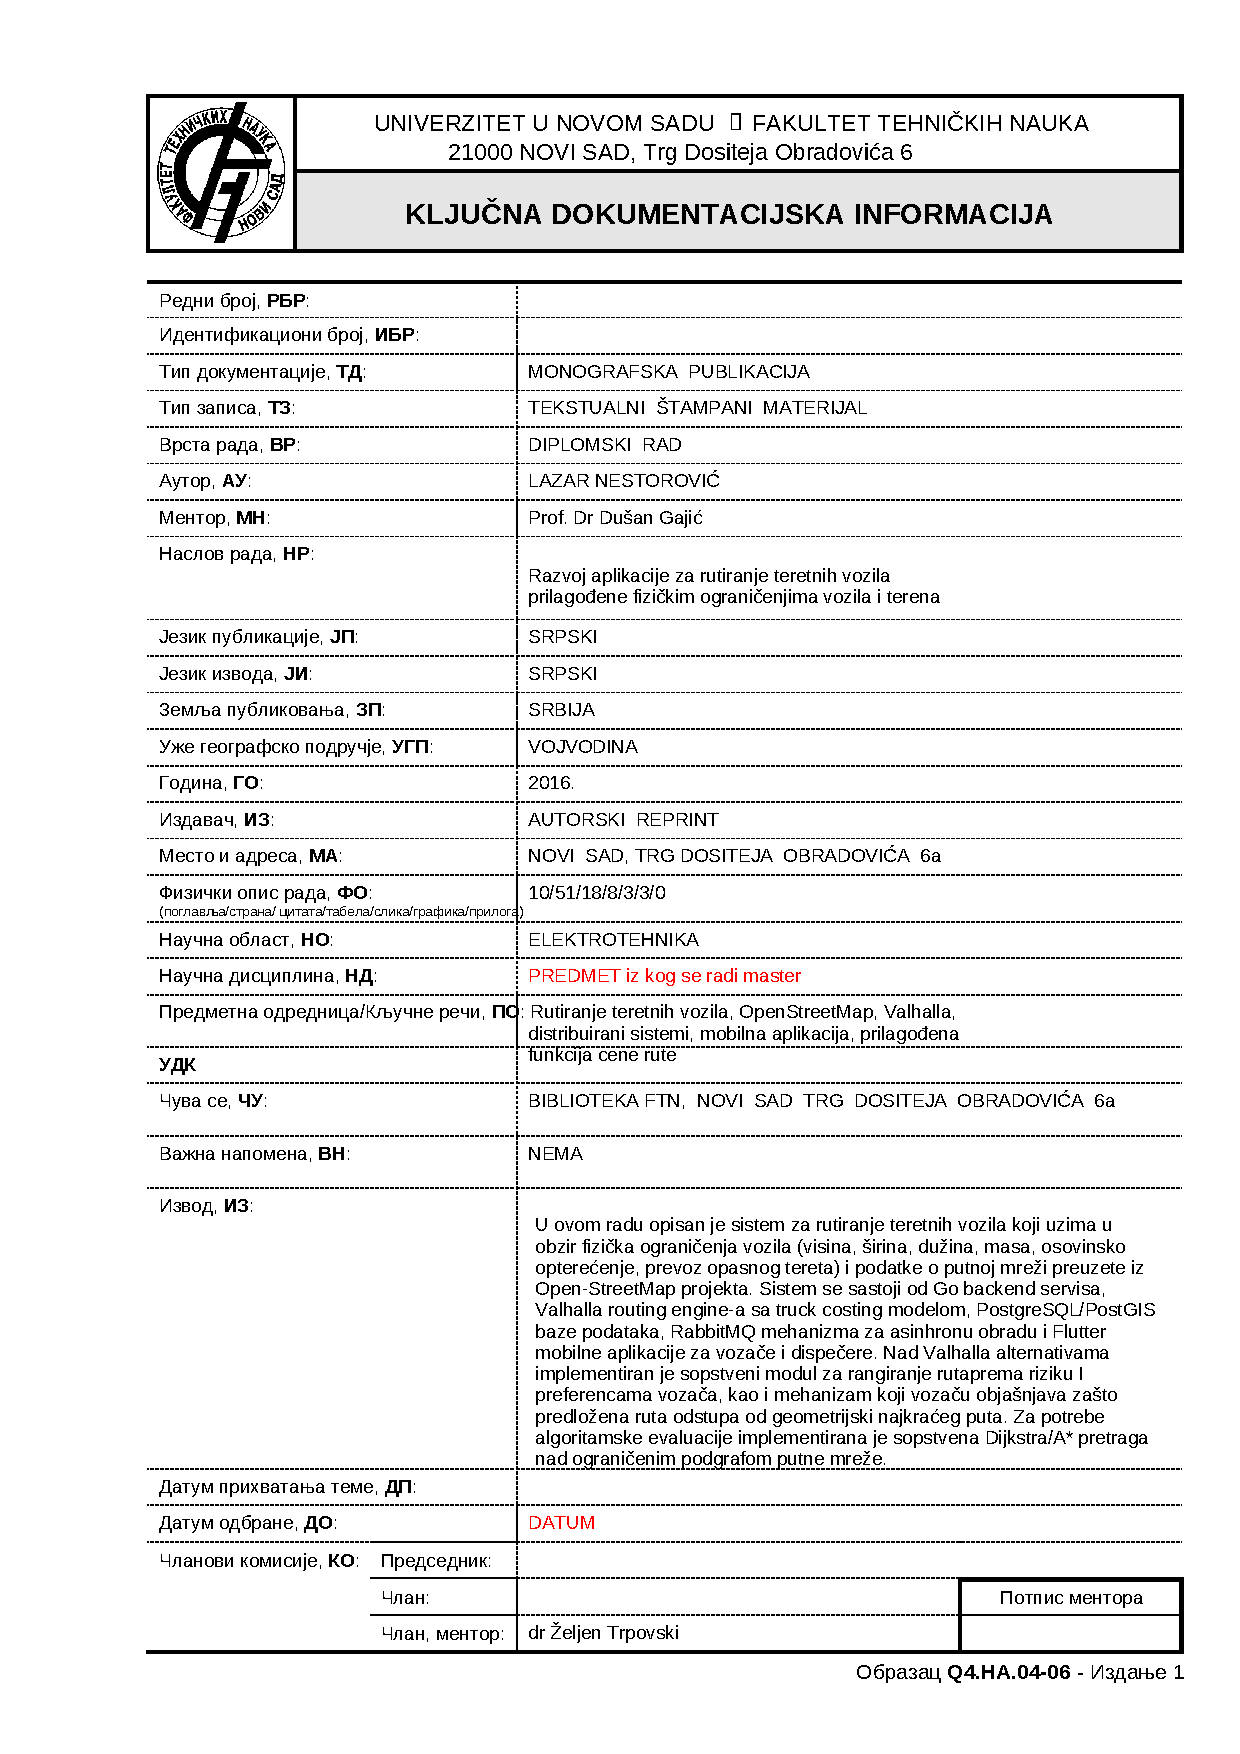
\includepdf[pages=1-2]{kljucna_dokumentacija_latinica.pdf} 
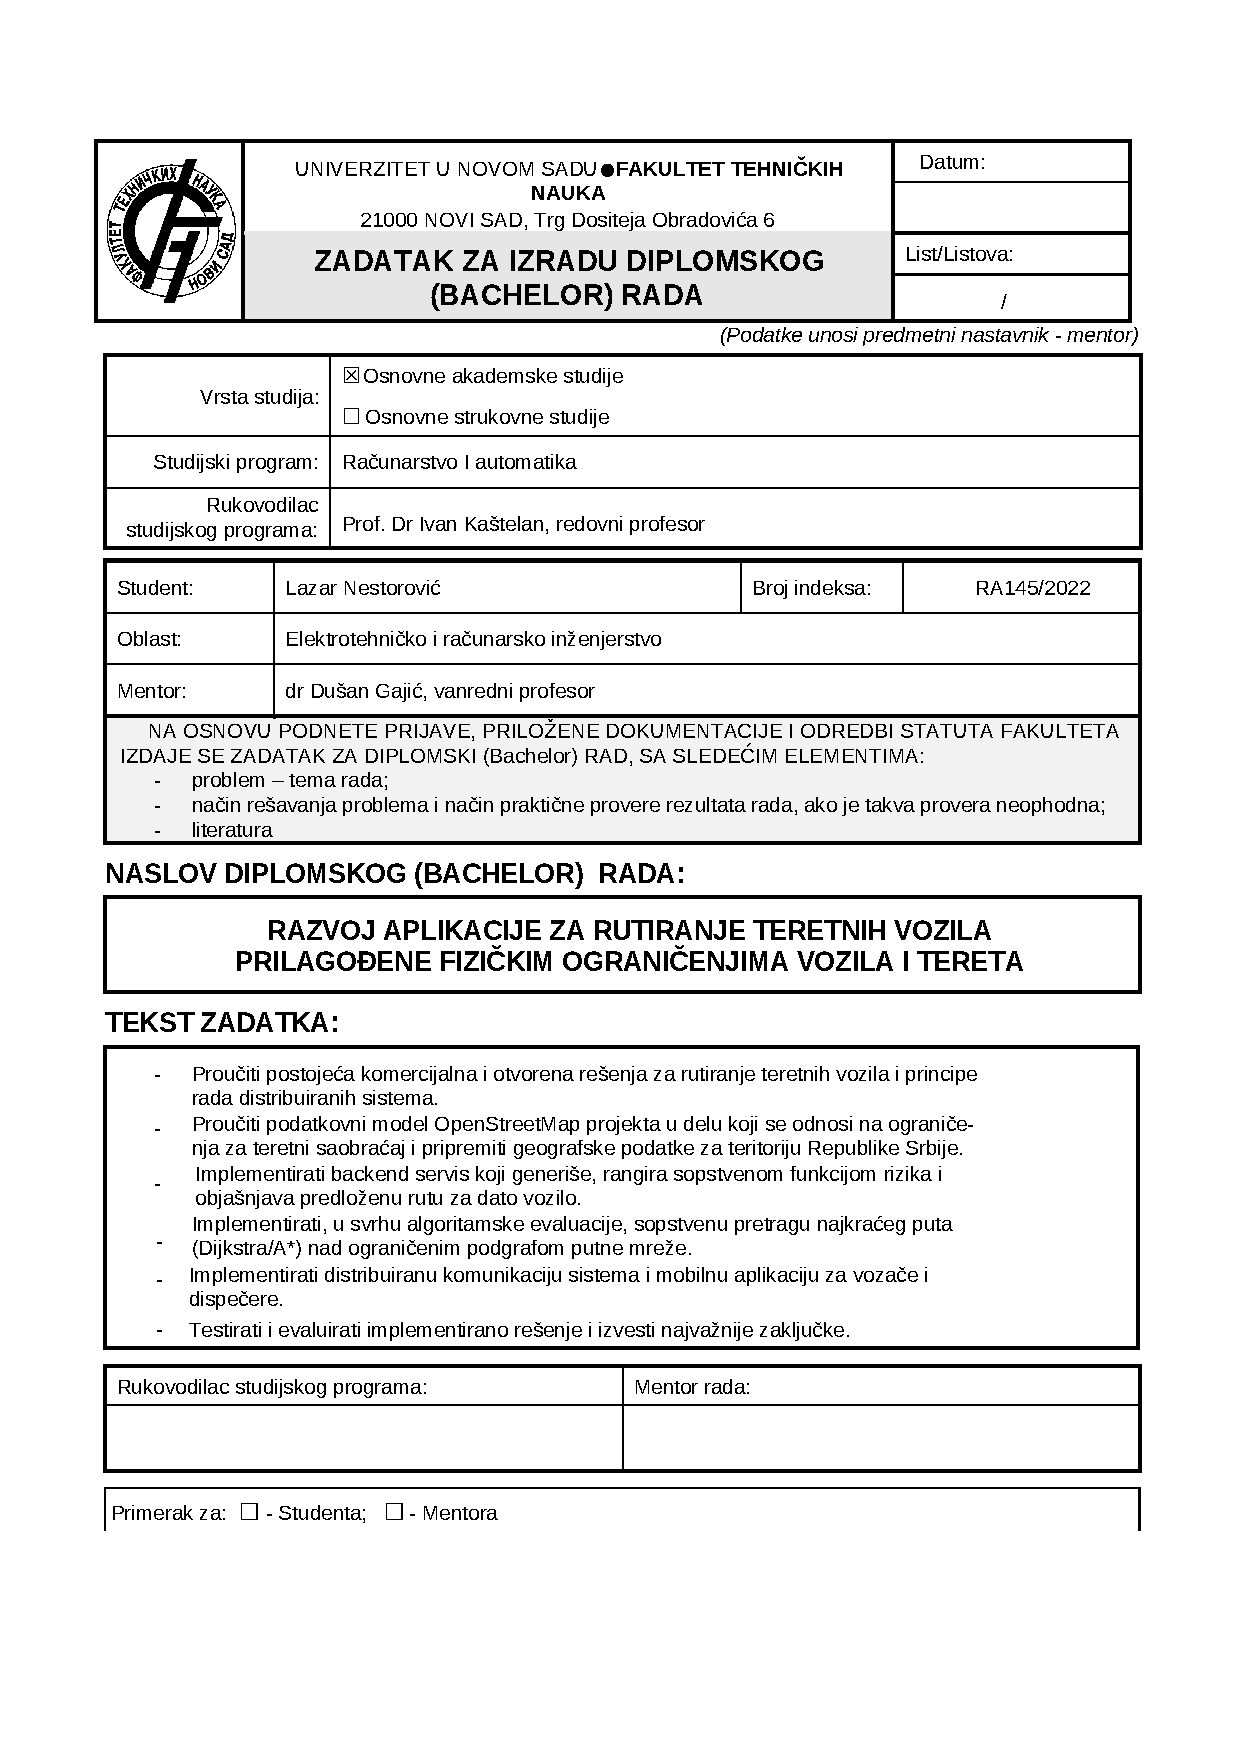
\includepdf[pages=1]{Zadatak_rada.pdf} 
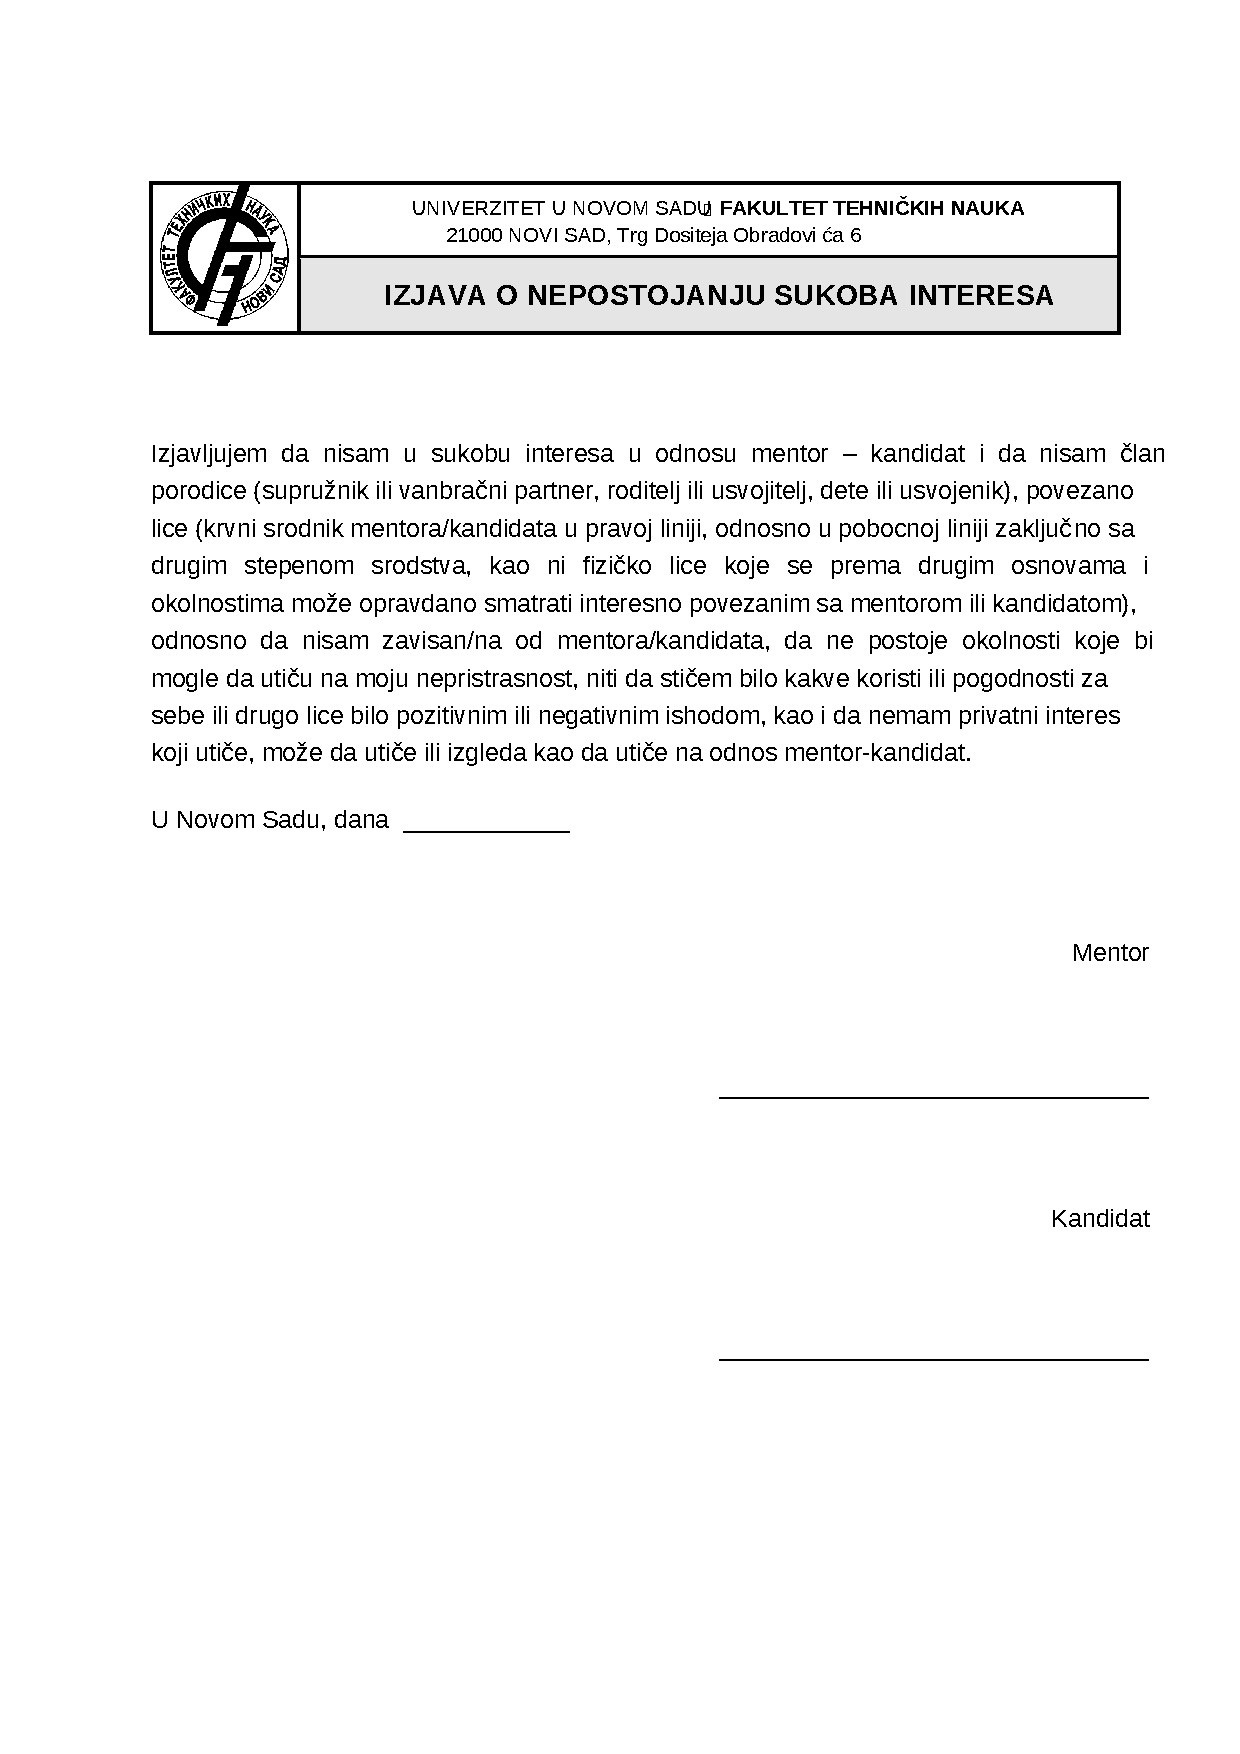
\includepdf[pages=1]{Izjava.pdf} 

\tableofcontents
\clearpage

\pagenumbering{arabic}
\chapter{Uvod}

Transport robe teškim teretnim vozilima podleže ograničenjima koja ne postoje kod putničkih automobila: visina vozila mora biti manja od visine svakog nadvožnjaka i tunela na ruti, ukupna masa i osovinsko opterećenje moraju biti u skladu sa nosivošću mostova, širina i dužina vozila ograničavaju kretanje kroz uža naselja i oštre krivine, a vozila koja prevoze opasan teret moraju zaobilaziti određene deonice (tunele, naseljena mesta) po propisu. Standardne aplikacije za navigaciju namenjene putničkim vozilima (Google Maps, Waze i slične) te podatke ne uzimaju u obzir, pa ruta koju predlažu vozaču teretnog vozila može biti fizički neprohodna ili čak zakonski nedozvoljena za dato vozilo. Sa druge strane, postojeća komercijalna rešenja specijalizovana za teretni saobraćaj (npr. PTV navigator, Google Maps za dostavu, TomTom Truck) su zatvorena, plaćena i ne omogućavaju uvid u to \emph{zašto} je određena ruta izabrana, što otežava vozaču da proceni da li je predlog razuman.

Ovaj rad opisuje razvoj sistema za rutiranje teretnih vozila koji rešava taj problem korišćenjem otvorenih geografskih podataka projekta OpenStreetMap (OSM) i otvorenog routing engine-a Valhalla, koji već ima ugrađen model cene rute specifičan za teretna vozila (\emph{truck costing}), sposoban da isključi deonice koje ne zadovoljavaju ograničenja visine, mase, širine ili prevoza opasnog tereta datog vozila. Na tu osnovu je dodat sopstveni sloj koji:

\begin{enumerate}
\item rangira alternativne rute koje Valhalla vrati prema riziku i preferencama vozača (stil vožnje, osetljivost tereta, potrošnja goriva, favorizovane lokacije na mapi), pošto sam Valhalla to ne radi;
\item vozaču objašnjava \textbf{zašto} je predložena ruta odstupila od geometrijski najkraćeg puta, umesto da mu samo prikaže krajnji rezultat;
\item omogućava, kao samostalnu algoritamsku celinu odvojenu od produkcionog puta, sopstvenu implementaciju Dijkstra i A* pretrage najkraćeg puta nad ograničenim podgrafom putne mreže, radi demonstracije i evaluacije principa na kojima Valhalla interno počiva.
\end{enumerate}

Sistem je zamišljen ne samo kao alat za planiranje jedne rute, već kao kompletna, iako po obimu ograničena, distribuirana aplikacija za rad voznog parka: pored planiranja i praćenja pojedinačne ture, uveden je i model dispečera koji upravlja više vozača i vozila, mehanizam ponude i prihvatanja ture između dispečera i vozača, chat u realnom vremenu, praćenje pozicije vozila uživo preko WebSocket veze, dnevnik događaja tokom vožnje i jednostavan mehanizam predloga pauze vozača zasnovan na proteklom vremenu vožnje. Sistem se sastoji od Go backend servisa, PostgreSQL/PostGIS baze podataka, RabbitMQ posrednika poruka, Valhalla routing engine-a i Flutter mobilne aplikacije, a svi servisi su kontejnerizovani i pokreću se preko \texttt{docker-compose}.

\section{Motivacija}

Motivacija za rad proizlazi iz konkretnog, ponovljivog problema: standardna navigacija ne razlikuje teretno vozilo od putničkog automobila, dok specijalizovana komercijalna rešenja skrivaju logiku odabira rute od korisnika i po pravilu zahtevaju plaćenu licencu i vlasnički skup podataka o putnoj mreži. Cilj ovog rada je da pokaže da se prihvatljivo tačan i \textbf{objašnjiv} sistem za rutiranje teretnih vozila može izgraditi nad potpuno otvorenim podacima (OSM) i otvorenim routing engine-om (Valhalla), uz sopstveni algoritamski doprinos koji tim alatima nedostaje: procenu rizika rute specifičnu za teretni saobraćaj i automatsko objašnjenje odstupanja rute od očekivanog, najkraćeg puta.

\section{Ciljevi i obim rada}

Ciljevi rada su:

\begin{itemize}
\item proučiti postojeća rešenja za rutiranje teretnih vozila i teorijske osnove distribuiranih sistema i algoritama pretrage najkraćeg puta u grafu;
\item pripremiti geografske podatke za teritoriju Republike Srbije iz OSM ekstrakta, sa oznakama relevantnim za teretni saobraćaj;
\item implementirati backend servis koji generiše, rangira i objašnjava rutu za dato vozilo, koristeći Valhallu kao routing engine;
\item implementirati, kao odvojenu algoritamsku celinu, sopstvenu Dijkstra/A* pretragu nad ograničenim podgrafom, radi evaluacije principa rutiranja bez zavisnosti od Valhalla-e;
\item implementirati distribuiranu komunikaciju sistema (REST, asinhrona obrada, WebSocket) i mobilnu aplikaciju za vozače i dispečere;
\item testirati implementirano rešenje i evaluirati doprinos sopstvene funkcije rizika u odnosu na "sirov" izbor rute.
\end{itemize}

Rad se svesno ne bavi punom implementacijom evropske AETR regulative o radnom vremenu i pauzama vozača, elevacionim (nagibnim) rizikom rute, offline režimom rada mobilne aplikacije, podrškom za više država niti bezbednosnim hardeningom na produkcionom nivou — ta ograničenja su namerna i obrazložena u poglavlju 10.

\section{Struktura rada}

Poglavlje 2 daje pregled postojećih komercijalnih i otvorenih rešenja za rutiranje teretnih vozila i teorijske osnove (distribuirani sistemi, algoritmi pretrage najkraćeg puta, OSM podatkovni model).\\Poglavlje 3 opisuje korišćene tehnologije.\\Poglavlje 4 opisuje arhitekturu sistema. \\Poglavlje 5 opisuje pripremu geografskih podataka.\\Poglavlje 6 detaljno opisuje algoritamski deo rada — Valhalla truck costing, sopstvenu funkciju rizika, mehanizam objašnjenja rute i sopstvenu Dijkstra/A* implementaciju. \\Poglavlje 7 opisuje backend servis i model podataka. \\Poglavlje 8 opisuje mobilnu aplikaciju. \\Poglavlje 9 opisuje testiranje i evaluaciju. \\Poglavlje 10 sadrži zaključak i pravce budućeg rada.

\clearpage

\chapter{Pregled postojećih rešenja i teorijske osnove}

\section{Komercijalna i otvorena rešenja za rutiranje teretnih vozila}

Rutiranje teretnih vozila je specijalizovana varijanta opšteg problema pronalaženja puta u grafu, sa dodatnim skupom ograničenja koja zavise od fizičkih karakteristika vozila i tereta. Postojeća rešenja mogu se podeliti u tri grupe.

\textbf{Komercijalna rešenja sa vlasničkim podacima.} PTV navigator i PTV xServer (nemački proizvođač PTV Group) su industrijski standard u logistici teretnog saobraćaja u Evropi; koriste vlasnički skup podataka o putnoj mreži sa ručno unetim ograničenjima za kamione (visina mostova, zabrane za HGV — \emph{Heavy Goods Vehicle} — u naseljima i sl.) i naplaćuju se po licenci. TomTom Truck i pojedini moduli Google Maps Platform-a (Routes API sa parametrima vozila) rade na sličnom principu — visok nivo tačnosti podataka, ali zatvoren izvor, zatvorena cena rute i bez mogućnosti da se razumeju ili prilagode kriterijumi po kojima je ruta izabrana.

\textbf{Otvoreni routing engine-i.} OSRM (\emph{Open Source Routing Machine}), GraphHopper i Valhalla su tri najpoznatija otvorena routing engine-a koji rade nad OpenStreetMap podacima. OSRM je najbrži za rutiranje putničkih vozila (koristi \emph{contraction hierarchies}), ali njegova podrška za teretna vozila je ograničena i uglavnom se svodi na jednostavne profile bez finog podešavanja po osovinskom opterećenju. GraphHopper ima ugrađen \texttt{truck} profil sličan Valhalla-inom i dobru Java/JVM integraciju, ali slabiju podršku za alternativne rute i manje detaljan mehanizam maneuver-a u odgovoru. Valhalla, koji je razvio Mapzen (danas ga održava zajednica okupljena oko Valhalla projekta), izabran je za ovaj rad zbog tri razloga: (1) ima \emph{per-request} \texttt{truck} costing model koji prihvata visinu, širinu, dužinu, masu, osovinsko opterećenje i prevoz opasnog tereta kao parametre HTTP zahteva, bez potrebe da se engine iznova kompajlira ili graf iznova gradi za svako vozilo; (2) podržava vraćanje više alternativnih ruta (\texttt{alternates}) u jednom zahtevu, što je preduslov za sopstveni sloj rangiranja opisan u poglavlju 6; (3) odgovor sadrži dovoljno detalja o maneuver-ima (tip, naziv ulice, početni indeks u geometriji rute) da se nad njim može izgraditi mehanizam objašnjenja rute (poglavlje 6.3) bez potrebe za dodatnim pozivima ka engine-u.

\textbf{Akademski i istraživački radovi.} Problem rutiranja vozila sa ograničenjima (\emph{constrained vehicle routing}) je dobro proučen u okviru šire oblasti \emph{Vehicle Routing Problem} (VRP) \cite{vrp} i njenih varijanti, gde se ograničenja tipično modeluju kao tvrda isključenja grana grafa (vozilo ne može da koristi granu) ili kao dodatni članovi u funkciji cene puta. Ovaj rad se ne bavi klasičnim VRP problemom (raspoređivanjem više vozila na više tura radi minimizacije ukupnog troška flote), već užim problemom rutiranja jednog vozila između dve tačke uz fizička ograničenja i sopstvenu procenu rizika — najbliži akademski okvir je \emph{constrained shortest path} problem, koji je u poglavlju 2.3 i 6.4 rešen sopstvenom implementacijom Dijkstra i A* algoritma sa isključivanjem grana koje vozilo ne može fizički da koristi.

Tabela 2.1 sumira poređenje.

\setlength{\tabcolsep}{4pt}
\renewcommand{\arraystretch}{1.3}

\begin{longtable}{@{}|p{0.148\textwidth}|p{0.148\textwidth}|p{0.148\textwidth}|p{0.148\textwidth}|p{0.148\textwidth}|p{0.148\textwidth}|@{}}
\caption{Poređenje pristupa rutiranju teretnih vozila}\label{tab:2-1}\\
\hline
\rowcolor{black!12}
\textbf{Rešenje} & \textbf{Izvor\newline podataka} & \textbf{Truck\newline costing} & \textbf{Alternative rute} & \textbf{Objašnjenje rute} & \textbf{Cena} \\
\hline
\endhead
PTV navigator / xServer & Vlasnički & Da, detaljan & Da & Ne (crna kutija) & Komercijalna licenca \\
\hline
Google Routes API (vozilo) & Vlasnički & Delimično & Da & Ne & Po pozivu (plaćeno) \\
\hline
OSRM & OSM & Ograničen & Da & Ne & Besplatno (open source) \\
\hline
GraphHopper & OSM & Da & Ograničeno & Ne & Besplatno / komercijalna podrška \\
\hline
Valhalla (bez izmena) & OSM & Da, detaljan & Da & Ne & Besplatno (open source) \\
\hline
\textbf{Ovaj rad (Valhalla+ sopstveni sloj)} & OSM & Da (Valhalla) & Da (Valhalla) & \textbf{Da (sopstveni modul)} & Besplatno \\
\hline
\end{longtable}

\setlength{\tabcolsep}{6pt}
\renewcommand{\arraystretch}{1}

\section{Distribuirani sistemi — osnovni pojmovi}

Sistem opisan u ovom radu je, u smislu klasifikacije koju daju Tanenbaum i van Steen \cite{tanenbaum}, \textbf{distribuiran sistem}: skup nezavisnih računarskih procesa (Go backend, PostgreSQL, RabbitMQ, Valhalla, Flutter klijenti) koji korisniku deluju kao jedinstvena celina, iako fizički i procesno rade odvojeno, najčešće u sopstvenim kontejnerima. U nastavku su ukratko definisani pojmovi neophodni za razumevanje arhitekture opisane u poglavlju 4 i 7.

\textbf{Model klijent-server.} Osnovni obrazac komunikacije u sistemu: mobilna aplikacija (klijent) šalje HTTP zahtev Go backend servisu (server), koji obrađuje zahtev i vraća odgovor. Sam backend je, u odnosu na Valhallu i bazu podataka, istovremeno klijent — što je uobičajena situacija u slojevitim sistemima, gde jedan proces može biti server u jednoj interakciji i klijent u drugoj.

\textbf{Sinhrona i asinhrona komunikacija.} REST API poziv je \emph{sinhron}: klijent čeka odgovor servera pre nego što nastavi. Za operacije koje ne moraju biti završene odmah da bi klijent nastavio sa radom (npr. proračun predloga pauze vozača nakon što je tura započeta), koristi se \emph{asinhroni} model preko posrednika poruka (RabbitMQ) — proizvođač (backend) objavljuje poruku o događaju i odmah nastavlja dalje, a potrošač (worker proces) je obrađuje kad je slobodan, nezavisno od toga da li je klijent koji je pokrenuo turu još povezan.

\textbf{Model izdavač-pretplatnik (publish–subscribe).} RabbitMQ u ovom sistemu radi kao \emph{topic exchange}: proizvođači objavljuju poruke sa određenim \emph{routing key}-em (npr. \texttt{trip.started}), a potrošači se pretplaćuju na red vezan za taj routing key. Ovaj model referencijalno razdvaja proizvođača od potrošača — backend koji objavljuje \texttt{trip.started} ne mora znati ništa o tome ko (ili da li uopšte neko) sluša taj događaj, što olakšava dodavanje novih potrošača bez izmene postojećeg koda (detaljnije u poglavlju 7.4).

\textbf{Real-time komunikacija (WebSocket).} REST model zahteva da klijent inicira svaki zahtev, što ga čini neprikladnim za slanje podataka od servera ka klijentu bez zahteva (npr. pozicija vozila koja se menja svake sekunde). WebSocket protokol (RFC 6455 \cite{websocket}) rešava taj problem uspostavljanjem trajne, dvosmerne veze preko jednog TCP soketa nakon početnog HTTP \emph{upgrade} zahteva — server u svakom trenutku može poslati poruku klijentu bez čekanja na njegov zahtev. U ovom sistemu se koristi za praćenje pozicije vozila uživo i za dopisivanje (chat) u realnom vremenu (poglavlje 7.5).

\textbf{Transparentnost i pouzdanost.} Od četiri klasična cilja distribuiranog sistema — povezanost, transparentnost, otvorenost i skalabilnost \cite{tanenbaum} — u ovom radu je najrelevantnija \emph{transparentnost otkaza} (\emph{fault transparency}): sistem je dizajniran da otkaz jedne komponente (npr. privremeni gubitak RabbitMQ konekcije od strane worker procesa) ne obori ostatak sistema, već da se poruka ponovo isporuči (\emph{message redelivery}, videti poglavlje 7.4) kada se komponenta ponovo poveže. S obzirom na obim rada (jedan backend, jedna baza, jedan message broker — bez replikacije ijedne komponente), sistem ne postiže skalabilnost po veličini u produkcionom smislu, što je namerno ograničenje obrazloženo u poglavlju 10.

\section{Grafovi i algoritmi najkraćeg puta}

Putna mreža se prirodno modeluje kao usmereni, težinski graf $G = (V, E)$, gde skup čvorova $V$ predstavlja tačke na putu (raskrsnice, prelome geometrije), a skup grana $E$ predstavlja segmente puta između susednih čvorova, sa težinom koja predstavlja cenu prelaska te grane (najčešće rastojanje u metrima, vreme u sekundama ili neka izvedena veličina). Problem rutiranja se svodi na pronalaženje puta $P$ od početnog čvora $s$ do ciljnog čvora $t$ koji minimizuje zbir težina grana na putu, uz eventualna dodatna ograničenja (izuzete grane).

\textbf{Dijkstra algoritam.} Dijkstrin algoritam \cite{dijkstra} pronalazi najkraći put od jednog čvora do svih ostalih čvorova u grafu sa nenegativnim težinama grana, koristeći greedy pristup: u svakom koraku bira neposećeni čvor sa najmanjom trenutno poznatom cenom od početka, "fiksira" tu cenu kao konačnu i ažurira cene njegovih suseda (\emph{relaxation}). Algoritam se efikasno implementira uz prioritetni red (u ovom radu binarna gomila, \texttt{container/heap} iz Go standardne biblioteke), sa vremenskom složenošću $O((|V| + |E|)\log|V|)$. Kada je poznat samo jedan ciljni čvor (a ne svi čvorovi grafa), pretraga se može prekinuti čim je ciljni čvor skinut sa reda — ta optimizacija je korišćena u implementaciji opisanoj u poglavlju 6.4.

\textbf{A*\emph{ algoritam.} A*} algoritam \cite{astar} je uopštenje Dijkstre koje uvodi \emph{heuristiku} $h(n)$ — procenu preostale cene od čvora $n$ do cilja — i usmerava pretragu prioritetno ka čvorovima za koje je zbir $f(n) = g(n) + h(n)$ (stvarna cena do sada plus procena preostale cene) najmanji. Ako je heuristika \emph{dopustiva} (nikad ne preceni stvarnu preostalu cenu), A* garantovano pronalazi optimalan put, uz manji broj posećenih čvorova od Dijkstre u praksi. U ovom radu je kao heuristika korišćena haversine udaljenost (linija vazdušne udaljenosti po sferi Zemlje) od trenutnog čvora do cilja, podeljena maksimalnom mogućom brzinom kretanja po grani — dopustiva heuristika jer nikad ne potcenjuje stvarni put duž putne mreže, koji je uvek duži ili jednak vazdušnoj liniji.

\textbf{Ograničena (constrained) pretraga.} Fizička ograničenja vozila (visina, masa, prevoz opasnog tereta) se u ovom radu modeluju kao \emph{tvrda isključenja} grane iz pretrage: grana koja ne zadovoljava profil vozila jednostavno se ne razmatra kao prelaz, čime pretraga po definiciji nikad ne predloži fizički neprohodnu rutu. Ovaj princip je identičan principu na kome interno počiva Valhalla-in \texttt{truck} costing model — razlika je u tome da Valhalla ta isključenja primenjuje nad grafom cele putne mreže, obogaćenim brojnim heuristikama (vreme prolaska, tipovi puta, istorijski podaci o saobraćaju), dok sopstvena implementacija u ovom radu (poglavlje 6.4) to radi nad znatno manjim, ograničenim podgrafom, isključivo radi transparentne demonstracije mehanizma.

\section{OpenStreetMap podatkovni model i oznake za teretni saobraćaj}

OpenStreetMap (OSM) je projekat slobodne, uređivačke geografske baze podataka sveta, u kojoj se putna mreža, objekti i granice modeluju preko tri osnovna geometrijska primitiva: \textbf{node} (tačka, definisana geografskom širinom i dužinom), \textbf{way} (uređena lista node-ova, predstavlja liniju ili poligon — npr. jedan segment puta) i \textbf{relation} (grupisanje node-ova, way-eva i drugih relation-a — npr. skup segmenata koji zajedno predstavljaju jednu magistralnu rutu ili ograničenje skretanja). Svaki od ova tri primitiva može imati proizvoljan skup \textbf{tag}-ova — parova ključ-vrednost koji opisuju njegova svojstva.

Za teretni saobraćaj relevantni su, između ostalih, sledeći tagovi (dokumentovani na OSM Wiki-ju \cite{osmwiki}):

\begin{itemize}
\item \texttt{maxheight}, \texttt{maxweight}, \texttt{maxwidth} — na way-u, ograničenje visine/mase/širine za tu deonicu (npr. nadvožnjak, tunel);
\item \texttt{hgv} — da li je way dozvoljen za teška teretna vozila (\emph{Heavy Goods Vehicle}), sa vrednostima poput \texttt{yes}, \texttt{no}, \texttt{destination};
\item \texttt{hazmat} — ograničenje za vozila koja prevoze opasan teret;
\item \texttt{maxaxleload} — ograničenje osovinskog opterećenja, relevantno za mostove;
\item \texttt{surface} — vrsta podloge (asfalt, kolovoz, tucanik i sl.), indirektno relevantno za rizik (loša podloga + veliko opterećenje = veći rizik);
\item \texttt{barrier} na node-u (npr. \texttt{barrier=height\_restrictor}, \texttt{barrier=lift\_gate}) — tačkasta prepreka koja može imati sopstveni \texttt{maxheight} tag, različit od tag-a way-a na kome se nalazi (npr. rampa niske visine na inače visokom putu);
\item \texttt{amenity=fuel}, \texttt{amenity=parking}, \texttt{highway=rest\_area} — node-ovi koji predstavljaju benzinske stanice, parkinge i odmarališta, relevantni za modul predloga pauze vozača (poglavlje 7.4).
\end{itemize}

Bitna karakteristika OSM podataka, relevantna za poglavlje 5, je da su ograničenja poput \texttt{maxheight} i \texttt{barrier} gotovo uvek zavedena na \textbf{way} nivou (za deonicu puta), dok su tačkaste prepreke (rampe, stubovi) zavedene na \textbf{node} nivou — što znači da alat koji filtrira OSM ekstrakt mora eksplicitno čuvati oba tipa tagova (way i node), jer se u suprotnom gubi tačno ona informacija koja je najrelevantnija za bezbednost teretnog vozila.

\clearpage

\chapter{Korišćene tehnologije}

\section{Go}

Backend servis je implementiran u programskom jeziku Go (Golang) \cite{go}, koji je razvio Google 2009. godine. Go je statički tipiziran, kompajliran jezik sa automatskim upravljanjem memorijom (\emph{garbage collection}) i ugrađenom podrškom za konkurentno programiranje preko \emph{goroutine}-a (lakih, korisnički upravljanih niti) i \emph{channel}-a (tipiziranih kanala za komunikaciju između goroutine-a). Za ovaj rad je Go izabran iz tri razloga: (1) standardna biblioteka već sadrži kompletan HTTP server (\texttt{net/http}, uz Go 1.22+ rutiranje po putanji i HTTP metodu preko \texttt{http.ServeMux}, korišćeno u \texttt{httpapi} paketu), bez potrebe za eksternim veb okvirom; (2) goroutine model konkurentnosti je pogodan za istovremeno opsluživanje mnogo WebSocket konekcija (poglavlje 7.5) i pozadinskog RabbitMQ potrošača (poglavlje 7.4) unutar istog procesa, bez složene infrastrukture za konkurentnost kakva bi bila potrebna u jednonitskim okruženjima; (3) statička tipizacija i kompajliranje u jedan izvršni fajl pogoduju jednostavnom kontejnerizovanju (poglavlje 3.7).

\section{Flutter i Dart}

Mobilna aplikacija je implementirana u Flutter okviru \cite{flutter}, koji koristi programski jezik Dart (oba razvijena od strane Google-a). Flutter kompajlira aplikaciju u nativni kod za Android i iOS iz jedinstvene baze izvornog koda, a korisnički interfejs se ne oslanja na nativne widgete platforme već na sopstveni \emph{rendering engine} (Skia/Impeller), čime se postiže vizuelna konzistentnost između platformi. Za potrebe ovog rada korišćene su, između ostalih, biblioteke \texttt{geolocator} (pristup GPS senzoru uređaja), \texttt{flutter\_map} odnosno OSM/vector tile prikaz mape, \texttt{web\_socket\_channel} za WebSocket konekcije i \texttt{google\_sign\_in} za prijavu preko Google naloga.

\section{Valhalla}

Valhalla \cite{valhalla} je otvoreni (open source) routing engine specijalizovan za rad nad OpenStreetMap podacima, originalno razvijen u kompaniji Mapzen. Za razliku od routing engine-a koji graf i cenu puta fiksiraju u trenutku izgradnje (tzv. \emph{preprocessing}, kakav koristi npr. OSRM sa \emph{contraction hierarchies}), Valhalla dozvoljava da se većina parametara cene puta (costing) prosledi \textbf{po zahtevu} (\emph{per-request}), uključujući ceo \texttt{truck} profil vozila — što znači da nije potrebno iznova graditi graf niti pokretati novu instancu servisa za svako vozilo ili promenu profila. Valhalla graf se organizuje u hijerarhijske "pločice" (\emph{tiles}), izgrađene alatom \texttt{valhalla\_build\_tiles} iz \texttt{.osm.pbf} ekstrakta (poglavlje 5.2), a HTTP API (\texttt{valhalla\_service}) prihvata zahteve na endpoint-u \texttt{/route} sa JSON telom koje uključuje lokacije, tip costing modela (\texttt{truck}) i njegove opcije. Detaljna upotreba Valhalla-inog truck costing modela u ovom radu opisana je u poglavlju 6.1.

\section{PostgreSQL i PostGIS}

PostgreSQL je korišćen kao relaciona baza podataka za skladištenje vozila, vozača, tura i pratećih entiteta (poglavlje 7.2). PostGIS \cite{postgis} je ekstenzija za PostgreSQL koja dodaje geografske tipove podataka i prostorne upite (npr. "sve tačke u krugu od 3km oko date koordinate"). Iako trenutna implementacija čuva geometriju rute kao enkodovan tekstualni \emph{polyline} (a ne PostGIS \texttt{geometry} kolonu — videti poglavlje 7.2 i ograničenja u poglavlju 10), PostGIS ekstenzija je uključena u korišćenu Docker sliku (\texttt{postgis/postgis:16-3.4-alpine}) kao osnova za prostorne upite koje bi budući razvoj (npr. pretraga "najbliže odmaralište" direktno u bazi umesto u memoriji, poglavlje 7.4) mogao iskoristiti bez promene infrastrukture.

\section{RabbitMQ}

RabbitMQ \cite{rabbitmq} je posrednik poruka (\emph{message broker}) koji implementira AMQP 0-9-1 protokol. U ovom sistemu se koristi \emph{topic exchange} (razmenjivač po temi) nazvan \texttt{trip.events}: proizvođač (backend) objavljuje poruku sa \emph{routing key}-em \texttt{trip.started} kada vozač pokrene turu, a worker proces (poglavlje 7.4) je preuzima iz reda vezanog za taj routing key, obrađuje je i upisuje rezultat (predlog pauze) u bazu. RabbitMQ je izabran zbog ugrađene podrške za potvrdu obrade poruke (\emph{acknowledgment}) i automatsko ponovno slanje neuspešno obrađene poruke (\emph{requeue}), što sistemu daje otpornost na privremeni pad worker procesa bez gubitka podataka o događaju.

\section{WebSocket}

Za real-time komunikaciju (praćenje pozicije vozila uživo i chat) korišćena je biblioteka \texttt{gorilla/websocket} na backend strani i \texttt{web\_socket\_channel} na Flutter strani, obe implementacije WebSocket protokola (RFC 6455 \cite{websocket}) nad HTTP/1.1 \emph{upgrade} mehanizmom. Detalji implementacije dati su u poglavlju 7.5.

\section{Docker i docker-compose}

Svi serverski delovi sistema (Go backend, PostgreSQL, RabbitMQ, Valhalla) su kontejnerizovani Docker slikama \cite{docker} i orkestrisani preko \texttt{docker-compose}, alata koji na osnovu deklarativnog YAML fajla pokreće, povezuje u zajedničku mrežu i redosledom health-check zavisnosti startuje više kontejnera jednom komandom (\texttt{docker compose up}). Ovo omogućava da se ceo backend deo sistema pokrene na bilo kojoj mašini sa Docker-om instaliranim, bez ručne instalacije PostgreSQL-a, RabbitMQ-a ili Valhalla-e — što je posebno važno za predvidljivost demonstracije rada (poglavlje 9). Detalji konfiguracije dati su u poglavlju 4.2.

\section{Ostale biblioteke i servisi}

\begin{itemize}
\item \textbf{JWT (JSON Web Token, RFC 7519 \cite{jwt})} — format za autentifikacione tokene korišćen preko biblioteke \texttt{golang-jwt/jwt}, sa HS256 potpisom; nosi identitet vozača i broj verzije tokena (\texttt{token\_version}), koji se koristi za "odjavu sa svih uređaja" bez potrebe za posebnom listom opozvanih tokena (poglavlje 4.3).
\item \textbf{bcrypt} — algoritam za heširanje lozinki sa ugrađenom "solju" i podesivim faktorom rada, korišćen umesto čuvanja lozinki u čistom tekstu ili prostog heša.
\item \textbf{Google Sign-In / JWKS} — prijava preko Google naloga verifikuje se ručnom proverom Google-ovog ID token-a nad javnim skupom ključeva (JWKS) preko biblioteke \texttt{MicahParks/keyfunc}, bez uvođenja celog Firebase SDK-a kao zavisnosti.
\item \textbf{Nominatim \cite{nominatim}} — javni servis za geokodiranje (pretvaranje adrese u koordinate i obrnuto) projekta OpenStreetMap, korišćen za pretragu adresa u mobilnoj aplikaciji (poglavlje 7.1), sa ograničenjem brzine poziva (throttling) u skladu sa politikom korišćenja servisa.
\item \textbf{goose \cite{goose}} — alat za upravljanje migracijama šeme baze podataka preko numerisanih SQL fajlova (poglavlje 7.2), koji garantuje da se svaka migracija primeni tačno jednom.
\item \textbf{osmium-tool} — komandolinijski alat za filtriranje i obradu \texttt{.osm}/\texttt{.osm.pbf} fajlova, korišćen u pripremi geografskih podataka (poglavlje 5.1).
\end{itemize}

\clearpage

\chapter{Arhitektura sistema}

\section{Pregled arhitekture i tok podataka}

Sistem se sastoji od pet nezavisnih procesa: Flutter mobilne aplikacije (klijent, vozač ili dispečer), Go backend servisa (centralna tačka logike), Valhalla routing engine-a, PostgreSQL/PostGIS baze podataka i RabbitMQ posrednika poruka. Slika 4.1 prikazuje njihov međusobni odnos i osnovni tok podataka pri planiranju i praćenju jedne ture.

\begin{figure}[h]
\centering
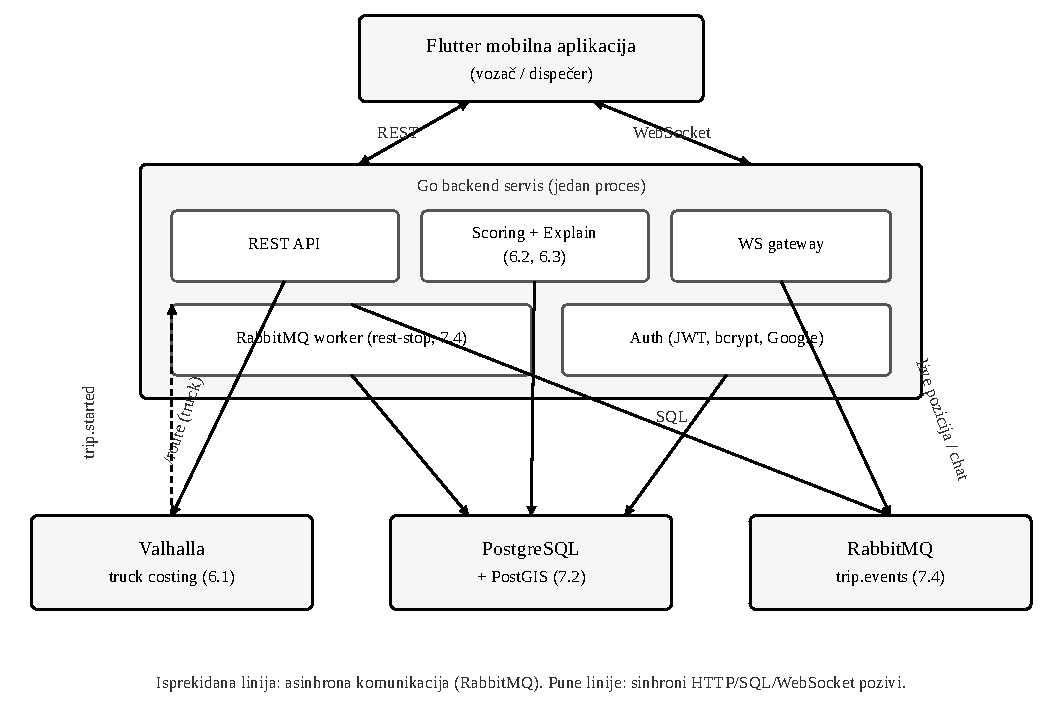
\includegraphics[width=0.88\textwidth]{diagrams/architecture.pdf}
\caption{Arhitektura sistema — komponente i tok podataka}
\label{fig:architecture}
\end{figure}

Tok pri planiranju rute je sledeći: mobilna aplikacija šalje \texttt{POST /api/v1/routes} sa profilom vozila, polazištem i odredištem; backend mapira profil vozila u Valhalla-in \texttt{truck} costing model (poglavlje 6.1) i traži do tri alternativne rute; svaka alternativa se rangira sopstvenom funkcijom rizika (poglavlje 6.2), a za izabranu (najbolje rangiranu) rutu se, ako odstupa od geometrijski najkraćeg puta, generiše tekstualno objašnjenje (poglavlje 6.3); odgovor sa geometrijom, rizikom i objašnjenjem se vraća klijentu. Kada vozač zaista pokrene turu (\texttt{POST /api/v1/trips}, zatim prelazak u status \texttt{in\_progress}), backend objavljuje \texttt{trip.started} događaj na RabbitMQ, koji worker procès preuzima i računa predlog pauze (poglavlje 7.4); istovremeno se otvara WebSocket veza (\texttt{GET /ws/trips/\{id\}}) preko koje se, dok vozač šalje periodične GPS pozicije (\texttt{POST /api/v1/trips/\{id\}/position}), te pozicije prosleđuju svim zainteresovanim klijentima uživo — vozačevom sopstvenom ekranu i, ako postoji, njegovom dispečeru koji sistem preko sopstvene, paralelne WebSocket konekcije prati na jednoj mapi (poglavlje 7.5, 8.2).

Sistem sledi troslojnu podelu odgovornosti sličnu klasičnoj veb arhitekturi \cite{tanenbaum}: sloj prezentacije (Flutter aplikacija), sloj obrade (Go backend, uključujući scoring i explain module) i sloj perzistencije (PostgreSQL). Razlika u odnosu na uobičajenu troslojnu veb aplikaciju je što backend za svaki zahtev za rutu sam postaje klijent eksternog servisa (Valhalla), a deo obrade (predlog pauze) je pomeren u nezavisan, asinhron proces (worker), radi rasterećenja glavne HTTP niti obrade zahteva.

\section{Kontejnerizacija i orkestracija servisa}

Svi serverski delovi sistema definisani su u jednom \texttt{docker-compose.yml} fajlu i pokreću se komandom \texttt{docker compose up}. Listing 4.1 prikazuje definiciju PostgreSQL servisa, sa health-check-om koji ostali servisi (backend) koriste kao uslov za sopstveni start preko \texttt{depends\_on: condition: service\_healthy} — čime se garantuje da backend ne pokuša konekciju na bazu koja još nije spremna za prihvat konekcija.

\begin{lstlisting}[caption={Definicija PostgreSQL/PostGIS servisa u \texttt{docker-compose.yml}}]
postgres:
  image: postgis/postgis:16-3.4-alpine
  environment:
    POSTGRES_USER: hvr
    POSTGRES_PASSWORD: hvr_dev_password
    POSTGRES_DB: hvr
  ports:
    - "5433:5432"
  volumes:
    - pgdata:/var/lib/postgresql/data
  healthcheck:
    test: ["CMD-SHELL", "pg_isready -U hvr -d hvr"]
    interval: 10s
    timeout: 5s
    retries: 5
\end{lstlisting}

Tabela 4.1 sumira sve servise definisane u \texttt{docker-compose.yml}, njihovu ulogu i portove koje izlažu na host mašini.

\begin{longtable}{@{}p{0.235\textwidth}p{0.235\textwidth}p{0.235\textwidth}p{0.235\textwidth}@{}}
\caption{Servisi definisani u \texttt{docker-compose.yml}}\label{tab:4-1}\\
\toprule
\textbf{Servis} & \textbf{Slika} & \textbf{Uloga} & \textbf{Port (host)} \\
\midrule
\endhead
\texttt{postgres} & \texttt{postgis/postgis:16-3.4-alpine} & Relaciona baza + PostGIS ekstenzija & 5433 → 5432 \\
\texttt{rabbitmq} & \texttt{rabbitmq:3-management-alpine} & Posrednik poruka (AMQP) + web konzola & 5672, 15672 \\
\texttt{valhalla} & \texttt{ghcr.io/valhalla/valhalla:latest} & HTTP routing servis (\texttt{valhalla\_service}) & 8002 \\
\texttt{valhalla-build} & \texttt{ghcr.io/valhalla/valhalla:latest} & Jednokratna izgradnja grafa iz OSM ekstrakta (profil \texttt{build}, ne pokreće se pri običnom \texttt{up}) & — \\
\texttt{backend} & sopstveni Go build & REST API, WebSocket gateway, worker & 8080 \\
\bottomrule
\end{longtable}

\texttt{valhalla-build} je definisan sa Docker Compose \emph{profilom} \texttt{build}, što znači da se ne pokreće automatski pri \texttt{docker compose up} — pokreće se izričito (\texttt{docker compose --profile build up valhalla-build}) samo kada treba ponovo izgraditi graf (npr. nakon promene OSM ekstrakta, poglavlje 5), i radi sa \texttt{network\_mode: none} jer mu za samu izgradnju grafa nije potrebna mrežna konekcija, čime se smanjuje površina za eventualni bezbednosni problem tog koraka. Mobilna aplikacija i sopstveni algoritamski modul (poglavlje 6.4) nisu deo \texttt{docker-compose.yml} — Flutter aplikacija se pokreće lokalno na razvojnoj mašini ili emulatoru, a algoritamski modul je čista Go biblioteka koja se pokreće isključivo kroz testove, bez sopstvenog servisa (obrazloženo u poglavlju 6.4).

\section{Sigurnost i autentifikacija}

Autentifikacija vozača i dispečera zasniva se na JWT tokenima (RFC 7519 \cite{jwt}) potpisanim HMAC SHA-256 algoritmom (HS256). Nakon prijave (\texttt{POST /auth/login} sa korisničkim imenom i lozinkom, ili \texttt{POST /auth/google} sa Google ID tokenom), backend izdaje token koji, pored identifikatora vozača, nosi i celobrojno polje \texttt{token\_version}. Ovo polje se upoređuje sa vrednošću \texttt{token\_version} iz baze na svakom autentifikovanom zahtevu (\texttt{RequireAuth} middleware) — kada vozač zatraži odjavu sa svih uređaja (\texttt{POST /auth/logout-all}), backend samo inkrementira \texttt{token\_version} u bazi, čime svi ranije izdati tokeni (koji nose stariju vrednost) trenutno postaju nevažeći, bez potrebe za posebnom, rastućom tabelom opozvanih tokena (\emph{blocklist}) koja bi morala da se proverava na svakom zahtevu.

Lozinke se ne čuvaju u čistom tekstu, već kao bcrypt heš, algoritam koji ugrađuje nasumičnu "sol" po lozinci (čime dve identične lozinke dva različita korisnika dobijaju različit heš) i podesivi faktor rada (koji direktno određuje koliko dugo traje jedan pokušaj heširanja, pa time i koliko dugo traje jedan pokušaj brute-force napada). Nalozi kreirani preko Google prijave nemaju lozinku (\texttt{password\_hash} je \texttt{NULL}) — identifikuju se preko stabilnog Google identifikatora naloga (\texttt{google\_sub}, \texttt{sub} polje iz Google ID tokena), koji backend verifikuje samostalno preko Google-ovog javnog skupa ključeva (JWKS), bez uvođenja Firebase SDK-a kao zavisnosti.

Za obnovu zaboravljene lozinke (\texttt{POST /auth/forgot-password}) i verifikaciju email adrese (\texttt{GET /auth/verify-email}) koristi se model jednokratnog, vremenski ograničenog tokena zapisanog u posebnoj tabeli (\texttt{password\_reset\_tokens}, \texttt{email\_verification\_tokens}) sa poljima \texttt{expires\_at} i \texttt{used\_at} — link poslat emailom prestaje da važi i po isteku vremena i po jednokratnoj upotrebi, a backend razlikuje ta dva slučaja radi jasnije poruke korisniku. Slanje emaila (link za verifikaciju/reset) realizovano je preko \texttt{net/smtp} paketa iz Go standardne biblioteke, bez eksternog transakcionog email API-ja — servis je no-op (ne šalje ništa, samo zapisuje u log) ako promenljiva okruženja \texttt{SMTP\_HOST} nije podešena, čime ostatak sistema radi i bez konfigurisanog email servisa (npr. u razvojnom okruženju).

Sistem u trenutnom obliku ima namerno ograničen bezbednosni obim, obrazložen u poglavlju 10 — WebSocket \texttt{CheckOrigin} provera je trenutno propustljiva (prihvata sve origin-e), pošto je aplikacija zamišljena kao rad sa jednim poznatim, poverljivim klijentom (sopstvena Flutter aplikacija), a ne kao javni, višezakupčani (multi-tenant) servis.

\clearpage

\chapter{Priprema geografskih podataka — OSM ekstrakcija za teretna vozila u Srbiji}

\section{Izvor podataka i osmium filter}

Osnovni izvor geografskih podataka je Geofabrik-ov dnevno ažuriran ekstrakt OpenStreetMap podataka za Srbiju (\texttt{serbia-latest.osm.pbf}) \cite{geofabrik}, preuzet automatizovanim \texttt{update-osm.sh} skriptom koja, pored preuzimanja, provera integritet fajla preko MD5 kontrolne sume koju Geofabrik objavljuje uz sam ekstrakt. Kompletan \texttt{.osm.pbf} fajl za Srbiju sadrži ogroman broj tagova nepotrebnih za rutiranje teretnih vozila (npr. sve poljoprivredne parcele, granice popisnih krugova, turističke oznake), pa se filtrira alatom \texttt{osmium-tools} \cite{osmium} pre nego što se prosledi Valhalla-i.

Listing 5.1 prikazuje tačnu \texttt{osmium tags-filter} komandu korišćenu u projektu.

\begin{lstlisting}[caption={Osmium filter za ekstrakciju podataka relevantnih za teretni saobraćaj}]
osmium tags-filter \
  serbia-latest.osm.pbf \
  w/highway w/maxheight w/maxweight w/maxwidth \
  w/hgv w/hazmat w/bridge w/tunnel \
  w/surface w/maxspeed \
  n/amenity=fuel,parking n/highway=rest_area n/barrier \
  r/type=restriction \
  --output serbia-hvt.osm.pbf --overwrite
\end{lstlisting}

Filter čuva way-eve (\texttt{w/}) sa tagovima relevantnim za geometriju i ograničenja puta (\texttt{highway}, \texttt{maxheight}, \texttt{maxweight}, \texttt{maxwidth}, \texttt{hgv}, \texttt{hazmat}, \texttt{bridge}, \texttt{tunnel}, \texttt{surface}, \texttt{maxspeed}), relacije (\texttt{r/}) tipa \texttt{restriction} (ograničenja skretanja) i, što je bilo kritično ispraviti tokom razvoja (videti dalje u ovom poglavlju), node-ove (\texttt{n/}) sa tagovima \texttt{amenity=fuel}, \texttt{amenity=parking}, \texttt{highway=rest\_area} i \texttt{barrier}. Way i node su, kako je objašnjeno u poglavlju 2.4, dva različita nivoa na kojima OSM podaci nose ograničenja relevantna za teretna vozila — way-evi obično nose ograničenje za celu deonicu (npr. \texttt{maxheight} na mostu), a node-ovi tačkastu prepreku (npr. rampu ili stub na ulazu u parking).

\textbf{Napomena o razvoju filtera.} Prva verzija filtera korišćena u ranoj fazi razvoja sadržala je samo \texttt{w/} i \texttt{r/} pravila, bez ijednog \texttt{n/} pravila — što je značilo da su svi node-ovi sa \texttt{amenity=fuel}, \texttt{amenity=parking}, \texttt{highway=rest\_area} i \texttt{barrier} tagovima bili odbačeni pri filtriranju, iako su neophodni za modul predloga pauze vozača (poglavlje 7.4). Ovaj propust je otkriven i ispravljen tokom pripreme podataka za rad — dodavanjem tri \texttt{n/} pravila filtrirani fajl je narastao sa 68 121 223 na 68 402 528 bajtova, a Valhalla graf je ponovo izgrađen sa ispravljenim skupom podataka. Ovaj slučaj ilustruje opštu lekciju vezanu za pripremu OSM podataka: filter koji izgleda kompletan gledano samo kroz way tagove tiho odbacuje čitavu kategoriju informacija zavedenih na node nivou, a greška se ne manifestuje kao pad sistema već kao \emph{nedostajuća} funkcionalnost koja se lako previdi dok se posebno ne testira.

\section{Izgradnja Valhalla grafa}

Filtriran \texttt{.osm.pbf} fajl se prosleđuje alatu \texttt{valhalla\_build\_tiles}, koji ga parsira i izgrađuje hijerarhijski graf organizovan u pločice (\emph{tiles}) — trajni format koji Valhalla HTTP servis (\texttt{valhalla\_service}) učitava pri startu i koristi za sve naredne \texttt{/route} zahteve. Ovaj korak je u sistemu izdvojen u poseban Docker Compose servis (\texttt{valhalla-build}, poglavlje 4.2), koji se pokreće samo kada treba ponovo izgraditi graf, a ne pri svakom pokretanju sistema (jer izgradnja traje nekoliko minuta i, s obzirom na to da se OSM podaci ne menjaju u toku jedne demonstracije rada, nije potrebno da se ona izvršava pri svakom \texttt{docker compose up}).

Nakon ispravke filtera opisane u 5.1, ponovo izgrađen graf za teritoriju Republike Srbije sadrži 898 337 čvorova i 2 216 948 usmerenih ivica (grana). Ovaj graf koristi isključivo Valhalla, preko HTTP \texttt{/route} poziva (poglavlje 6.1) — nije direktno dostupan Go backend-u niti bilo kom drugom delu sistema, čime se čitava logika parsiranja OSM podataka i izgradnje efikasne rutne strukture prepušta Valhalla-i, u skladu sa odlukom (obrazloženom u poglavlju 6) da se produkcioni put ne oslanja na sopstvenu implementaciju pretrage nad grafom cele države.

\section{Ekstrakcija podataka o odmaralištima}

Za modul predloga pauze vozača (poglavlje 7.4) backend ne poziva Valhallu, već direktno učitava, pri pokretanju, sve node-ove sa tagovima \texttt{amenity=fuel}, \texttt{amenity=parking} i \texttt{highway=rest\_area} iz filtriranog OSM ekstrakta (istog fajla korišćenog za izgradnju Valhalla grafa, poglavlje 5.1) u memoriju procesa — oko 2000 node-ova za teritoriju Srbije. Ova lista se pri svakom predlogu pauze pretražuje geometrijski: kandidat mora biti unutar zadatog radijusa od tačke na ruti u kojoj bi vozilo teorijski bilo nakon isteka praga vožnje (poglavlje 7.4), i mora zaista biti u koridoru trase (a ne, na primer, geometrijski najbliža tačka vazdušnom linijom koja se nalazi na potpuno drugom putu). Rezultat pretrage dodatno favorizuje omiljene ili brend-specifične lokacije vozača, a za vozila koja prevoze opasan teret preferira benzinske stanice nad parkinzima u granicama tolerancije rastojanja — detalji ove logike dati su u poglavlju 7.4.

\clearpage

\chapter{Algoritam rutiranja prilagođen vozilu}

Ovo poglavlje je centralni algoritamski doprinos rada. Sistem koristi \textbf{dvoslojni pristup}: (1) u produkcionom putu, Valhalla generiše fizički dopustive alternativne rute preko svog \texttt{truck} costing modela (6.1), nad kojima sopstveni Go modul dodaje rangiranje po riziku (6.2) i objašnjenje odstupanja rute (6.3), pošto to Valhalla nativno ne radi; (2) kao odvojena, algoritamska celina namenjena evaluaciji i demonstraciji principa, implementirana je sopstvena Dijkstra/A* pretraga nad ograničenim podgrafom putne mreže, direktno nad OSM podacima, bez ikakve zavisnosti od Valhalla-e (6.4). Ovaj pristup je posledica realne procene obima rada: reimplementacija efikasnog nacionalnog routing engine-a nad grafom od skoro milion čvorova (poglavlje 5.2) nije realan cilj jednog diplomskog rada, dok je razumevanje i demonstracija principa na kojima takav engine počiva — kroz sopstvenu, testiranu implementaciju nad manjim, ali realnim podgrafom — sasvim ostvarivo i akademski relevantno.

\section{Valhalla truck costing}

Valhalla-in \texttt{truck} costing model prihvata profil vozila kao deo tela HTTP \texttt{/route} zahteva, bez potrebe da se graf iznova izgradi za svako vozilo. Listing 6.1 prikazuje tipičan zahtev korišćen u ovom sistemu.

\newpage
\begin{lstlisting}[caption={[Zahtev za truck-costed rutu sa alternativama]Zahtev za truck-costed rutu sa alternativama (visina/širina/dužina u metrima, masa/osovinsko opterećenje u tonama)}]
POST /route
{
  "locations": [
    {"lat": 44.8, "lon": 20.4},
    {"lat": 45.25, "lon": 19.85}
  ],
  "costing": "truck",
  "costing_options": {
    "truck": {
      "height": 4.0,
      "width": 2.55,
      "length": 16.5,
      "weight": 40,
      "axle_load": 11.5,
      "hazmat": false
    }
  },
  "alternates": 2
}
\end{lstlisting}

Backend mapira sopstveni \texttt{TruckProfile} (u SI jedinicama — metrima i kilogramima, radi konzistentnosti sa ostatkom sistema) u Valhalla-ine jedinice (metri za dimenzije, metrički toni za masu), i parsira odgovor u sopstvenu strukturu \texttt{RouteCandidate} koja, pored rastojanja i trajanja, izdvaja i broj manevara, udeo puta na magistralnim/autoputskim deonicama (\texttt{HighwayRatio}), prisustvo trajekta ili putarine, kao i nazive ulica i tačke svakog manevra — signale koje ne izlaže sam sažetak rute, ali su neophodni za sloj rangiranja (6.2) i objašnjenja (6.3). Listing 6.2 prikazuje deo implementacije koja šalje zahtev i mapira profil vozila.

\newpage
\begin{lstlisting}[caption={[Mapiranje profila vozila u Valhalla \texttt{costing\_options}]\texttt{valhalla.Client.RouteAlternates} — mapiranje profila vozila u Valhalla \texttt{costing\_options} (\texttt{backend/internal/valhalla/client.go})}]
// TruckProfile mirrors Valhalla's truck costing_options, in SI units (meters, kilograms).
type TruckProfile struct {
	HeightM    float64
	WidthM     float64
	LengthM    float64
	WeightKg   float64
	AxleLoadKg float64
	Hazmat     bool
}

func (c *Client) RouteAlternates(ctx context.Context, origin, destination LatLon,
	profile TruckProfile, numAlternates int) ([]RouteCandidate, error) {
	body := routeRequest{
		Locations: []LatLon{origin, destination},
		Costing:   "truck",
		CostingOptions: map[string]truckCostingOpt{
			"truck": {
				Height:   profile.HeightM,
				Width:    profile.WidthM,
				Length:   profile.LengthM,
				Weight:   profile.WeightKg / 1000,   // Valhalla expects metric tons
				AxleLoad: profile.AxleLoadKg / 1000,
				Hazmat:   profile.Hazmat,
			},
		},
		Alternates: numAlternates,
	}
	// ... serijalizacija, HTTP POST na baseURL+"/route", parsiranje odgovora
}
\end{lstlisting}

Ograničenje ovog pristupa je da odgovor običnog \texttt{/route} poziva ne izlaže \emph{koja tačno} ivica grafa je isključena niti njenu tačnu vrednost ograničenja (npr. tačnu visinu nadvožnjaka) — ta informacija bi zahtevala poziv Valhalla-inog \texttt{/trace\_attributes} endpoint-a nad već izračunatom rutom, ili direktan pristup OSM podacima nezavisno od Valhalla-e. Ovo ograničenje je direktno motivisalo modul opisan u 6.4, koji, radeći nad sopstvenim, manjim grafom, ima pristup tačnim OSM tagovima svake ivice.

\section{Prilagođena funkcija rizika (scoring)}

Valhalla po zahtevu vraća do tri alternativne rute, ali ih ne rangira po bilo kom kriterijumu specifičnom za teretni saobraćaj — sve tri su, sa njene tačke gledišta, fizički dopustive. Paket \texttt{scoring} dodaje taj nedostajući sloj: svaku alternativu boduje heurističkom funkcijom rizika koja kombinuje rastojanje, broj manevara, udeo puta van magistralnih deonica, prisustvo trajekta/putarine, procenu potrošnje goriva u odnosu na masu vozila, broj "oštrih" manevara (proxy za rizik pomeranja tereta) i blizinu omiljenih benzinskih stanica vozača — a zatim vraća alternative sortirane od najboljeg (najmanji rizik) ka najgorem rezultatu.

Svaka dimenzija skalira se prema preferenci vozača, izraženoj kao ceo broj od 1 do 5 (gde je 3 neutralna, podrazumevana vrednost) preko faktora \texttt{priority/3} — vozač koji nikad ne podesi svoje preference dobija rezultat identičan fiksnoj, uravnoteženoj formuli. Listing 6.3 prikazuje centralnu funkciju bodovanja.

\begin{lstlisting}[caption={[Funkcija bodovanja rute]Funkcija bodovanja rute (\texttt{backend/internal/scoring/scoring.go}) — manji rezultat je bolji}]
func score(c valhalla.RouteCandidate, prefs Preferences, vehicleWeightKg,
	fastestDurationMin float64, preferredStops []valhalla.LatLon) float64 {
	var timeTerm float64
	if fastestDurationMin > 0 {
		timeTerm = (c.DurationMin - fastestDurationMin) / fastestDurationMin * timeScale
	}
	highwayTerm := (1 - c.HighwayRatio) * nonHighwayScale
	fuelTerm := fuelProxy(c, vehicleWeightKg)
	cargoTerm := float64(c.SharpManeuverCount) * sharpManeuverWt

	s := scalar(prefs.TimePriority)*timeTerm +
		scalar(prefs.HighwayPriority)*highwayTerm +
		scalar(prefs.FuelPriority)*fuelTerm +
		scalar(prefs.CargoPriority)*cargoTerm +
		float64(c.ManeuverCount)*maneuverWeight

	if c.HasFerry {
		s += ferryPenalty
	}
	if c.HasToll {
		s += tollPenalty
	}
	s += preferredStopDiscount(c.Shape, preferredStops)
	return s
}
\end{lstlisting}

Vrednost \texttt{timeTerm} je relativno kašnjenje kandidata u odnosu na najbržeg kandidata u istom skupu alternativa (0\% ako je kandidat najbrži), a \texttt{fuelProxy} je relativna procena "potrošnje" izvedena iz rastojanja i mase vozila (nema pristupa podacima o nagibu puta, pa ovo nije stvarna potrošnja u litrima, već relativan signal za poređenje kandidata međusobno). Bazne težine (\texttt{maneuverWeight}, \texttt{nonHighwayScale}, \texttt{ferryPenalty} itd.) su prva heuristička procena, nekalibrisana prema stvarnim podacima o potrošnji ili nesrećama — što je namerno ograničenje, razmatrano dalje u poglavlju 9.3 kroz konkretan primer greške koju je ova formula ispravila.

\textbf{Motivacija dodavanja vremenskog člana.} Rana verzija formule nije sadržala \texttt{timeTerm} — bodovala je isključivo na osnovu udela magistralne deonice (\texttt{highwayTerm}) i broja manevara. Testiranjem na konkretnoj ruti (Radalj, poglavlje 9.3) uočeno je da takva formula bira rutu koja je 47\% duža i 30\% sporija od alternative samo zato što ima nešto povoljniji odnos magistralne i lokalne deonice puta — očigledno pogrešan ishod sa stanovišta stvarnog transportnog troška. Dodavanje \texttt{timeTerm}-a, koji direktno kažnjava kandidata srazmerno tome koliko je sporiji od najbržeg u skupu, ispravilo je taj slučaj bez uklanjanja postojećih članova formule.

\section{Objašnjenje predložene rute — slučaj Novi Banovci}

Kada izabrana ruta odstupa od geometrijski najkraćeg puta, vozaču nije dovoljno prikazati \emph{šta} je predloženo — potrebno mu je objašnjenje \emph{zašto}. Paket \texttt{explain} implementira taj mehanizam prema principu binarne pretrage po dimenzijama profila vozila:

\begin{enumerate}
\item Zahteva se "referentna" ruta sa svim dimenzijama profila veštački opuštenim na nerealno velike vrednosti (npr. visina 100m, masa 900 000 kg) — ruta koju bi Valhalla predložila da fizička ograničenja vozila ne postoje.
\item Ako se izabrana ruta (sa stvarnim profilom vozila) po rastojanju ne razlikuje značajno od referentne (manje od 1km), nema odstupanja koje treba objasniti.
\item U suprotnom, dimenzije profila (visina, masa, osovinsko opterećenje, širina, prevoz opasnog tereta) se redom, jedna po jedna, "oslobađaju" na referentnu vrednost, i ruta se ponovo traži — dimenzija čije oslobađanje vrati rutu na rastojanje referentne rute je \textbf{vezujuće ograničenje} za taj segment puta.
\item Mesto odstupanja se određuje geometrijski: dekodirane geometrije (polyline) izabrane i referentne rute se upoređuju tačku po tačku, a prva tačka izabrane rute čija je udaljenost od svake tačke referentne rute veća od 200m proglašava se tačkom divergencije; njoj se pridružuje naziv ulice najbližeg manevra izabrane rute.
\item Generiše se poruka vozaču, npr.: \emph{"Ruta skreće kod [ulica] jer visina vozila (4.7m) ne zadovoljava ograničenje na toj deonici."}
\end{enumerate}

\begin{figure}[h]
\centering
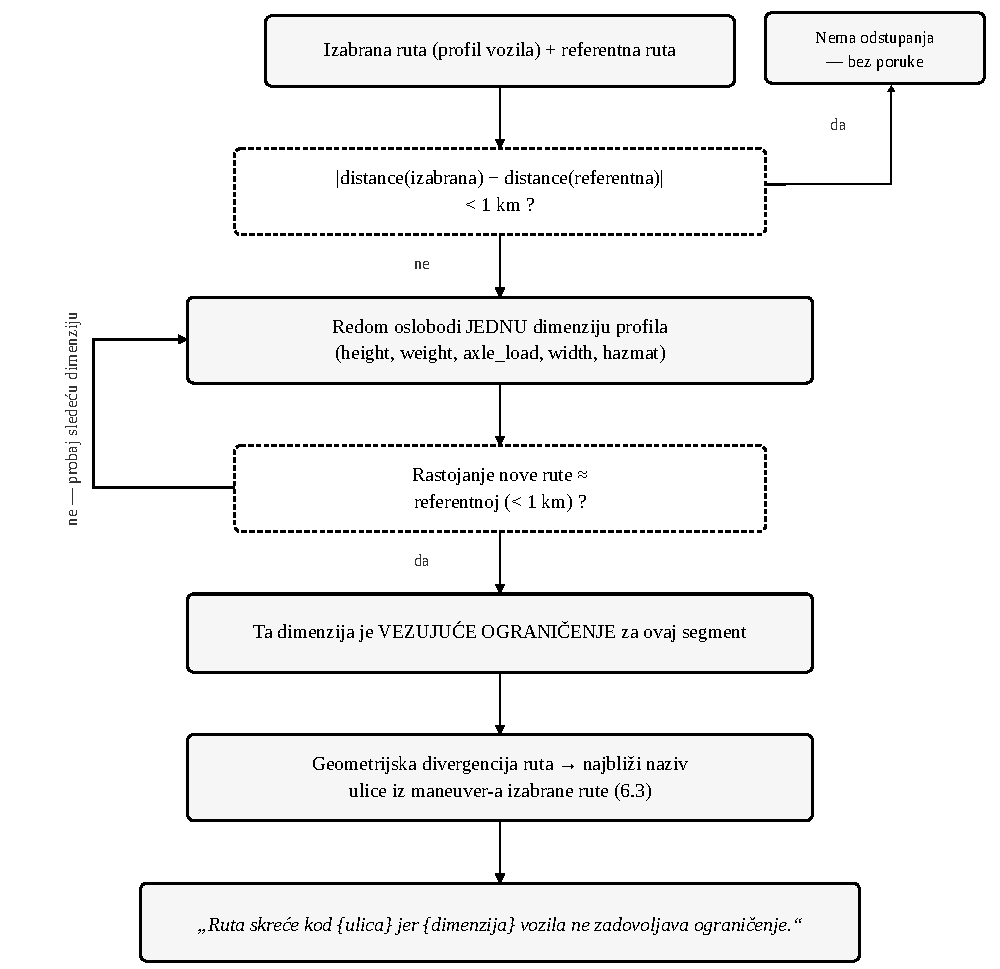
\includegraphics[width=0.88\textwidth]{diagrams/explain.pdf}
\caption{Tok mehanizma objašnjenja rute (\texttt{explain.Explain})}
\label{fig:explain}
\end{figure}

\textbf{Slučaj Novi Banovci.} Ovaj mehanizam je razvijen i potvrđen na konkretnom, stvarnom slučaju: ručnom binarnom pretragom (ponavljanjem \texttt{/route} poziva sa različitim vrednostima visine) utvrđeno je da na auto-putu A1, u okolini čvora Novi Banovci (izlaz 21/22), postoji ograničenje visine između 4.5m i 4.6m. Za vozilo profila korišćenog u testu (visina 4.7m), Valhalla je korektno birala detour preko lokalnog puta umesto direktnog nastavka auto-putem — a mehanizam opisan u ovom poglavlju automatizuje upravo tu istu binarnu pretragu, koju je autor prvo sproveo ručno da bi potvrdio da je ponašanje Valhalla-e (i, posledično, sistema) tačno.

Bitna napomena o ovom mehanizmu je da se poređenje izabrane i referentne rute sprovodi \textbf{isključivo geometrijski}, a ne nad strukturom odgovora koju vraća Valhalla. Umesto da se upoređuju liste manevara (\texttt{street\_names}) ili njihovi redni brojevi, dekodiraju se polyline geometrije obe rute i porede se same sekvence geografskih koordinata: za svaku tačku izabrane rute traži se najmanje rastojanje do bilo koje tačke referentne rute, a prva tačka kod koje to rastojanje pređe prag od 200m proglašava se tačkom divergencije. Prag od 200m je kompromis — dovoljno velik da apsorbuje razliku u gustini uzorkovanja tačaka između dve rute i sitna odstupanja u okviru istog koridora (npr. razdvojene kolovozne trake auto-puta), a dovoljno mali da stvarno skretanje na drugi put bude detektovano gotovo odmah po nastanku.

Prednost ovakvog pristupa je što ne pretpostavlja nikakvu korespondenciju između strukture dva odgovora. Dve rute do istog odredišta mogu imati potpuno različit broj manevara, različito imenovane ulice i različitu podelu puta na segmente, pa je svako poređenje zasnovano na poziciji u nizu pouzdano samo dok se rute uglavnom podudaraju. Kod vozila sa strogim ograničenjima Valhalla neretko bira globalno drugačiju strategiju rute od samog polaska, čime takva korespondencija u potpunosti nestaje. Geometrija, nasuprot tome, opisuje fizički položaj vozila na mreži i nezavisna je od načina na koji je ruta izdeljena na manevre — mesto gde se dve rute razilaze je uvek dobro definisano u prostoru, bez obzira na to kako je opisano u odgovoru. Nazivi ulica se zato koriste tek naknadno, i to samo kao \emph{oznaka} već pronađene tačke divergencije: nakon što je tačka geometrijski određena, njoj se pridružuje naziv prostorno najbližeg manevra izabrane rute, kako bi poruka vozaču bila razumljiva u terminima stvarne putne mreže.

\section{Sopstvena implementacija pretrage puta nad ograničenim podgrafom}

Kao samostalna algoritamska celina, odvojena od produkcionog puta (nije uvezana u \texttt{main.go} niti u REST API — koristi se isključivo kroz sopstvene testove), implementirana je sopstvena Dijkstra i A*\emph{ pretraga najkraćeg puta koja radi direktno nad OSM XML podacima, bez ikakve zavisnosti od Valhalla-e. Svrha ovog modula nije da zameni Valhallu u produkciji (poglavlje 5.2 objašnjava zašto bi reimplementacija efikasnog routing engine-a nad grafom cele države bila nerealan cilj za obim ovog rada), već da (a) demonstrira, kroz sopstveni, testiran kod, principe na kojima Valhalla interno počiva (isključivanje fizički nedopustivih grana, pretraga najkraćeg puta uz heuristiku), i (b) da posluži kao alat za evaluaciju i poređenje Dijkstra i A*} pristupa nad istim, realnim podacima (poglavlje 9.2), sa direktnim pristupom OSM tagovima koje obični Valhalla \texttt{/route} odgovor ne izlaže (poglavlje 6.1).

\textbf{Graf i model podataka.} Graf se učitava iz \texttt{.osm} (XML) ekstrakta funkcijom \texttt{LoadOSMXML}, koja parsira way-eve sa tagom \texttt{highway} u usmerene ivice (\texttt{Edge}), čuvajući po ivici dužinu, klasu puta (\texttt{RoadClass}), podlogu (\texttt{Surface}) i, ako postoje, ograničenja \texttt{maxheight}/\texttt{maxweight}/\texttt{hazmat} preuzeta sa way-a. Node-ovi koji imaju sopstveni \texttt{barrier} tag sa \texttt{maxheight}/\texttt{maxweight} (npr. rampa niže visine na inače prohodnom putu) čuvaju se kao ograničenje na samom čvoru (\texttt{Node.MaxHeightM}), odvojeno od ograničenja na ivici — jer, kako je objašnjeno u poglavlju 2.4, OSM te dve vrste ograničenja zavodi na dva različita nivoa.

\textbf{Funkcija cene.} Cena prelaska ivice je njena dužina u metrima, uvećana za faktor lošije podloge (\texttt{unpaved}, \texttt{gravel}, \texttt{dirt}, \texttt{sett} — 30\% penal) i skalirana faktorom preferencije klase puta (Tabela 6.1) — magistralni putevi i auto-putevi imaju blagi popust u ceni (manje raskrsnica/prilaza po kilometru za veliko vozilo), dok sekundarni putevi imaju blagi penal. Na svaki prelaz sa ivice na ivicu (skretanje) dodaje se i penal za oštrinu ugla skretanja, izražen u istoj jedinici ("metar") kao i osnovna cena, radi jednostavnog sabiranja — svi ovi koeficijenti su, kao i kod paketa \texttt{scoring} (6.2), heuristička, nekalibrisana prva procena, što je u kodu izričito dokumentovano.

\begin{longtable}{@{}p{0.470\textwidth}p{0.470\textwidth}@{}}
\caption{Faktor preferencije klase puta (\texttt{roadClassMultiplier})}\label{tab:6-1}\\
\toprule
\textbf{Klasa puta (OSM \texttt{highway})} & \textbf{Faktor} \\
\midrule
\endhead
\texttt{motorway} & 0.85 \\
\texttt{motorway\_link} & 0.90 \\
\texttt{trunk} & 0.90 \\
\texttt{trunk\_link} & 0.95 \\
\texttt{primary} & 1.00 \\
\texttt{primary\_link} & 1.05 \\
\texttt{secondary} & 1.15 \\
\texttt{secondary\_link} & 1.20 \\
\bottomrule
\end{longtable}

Listing 6.4 prikazuje isključivanje nedopustivih ivica i čvorova (tvrdo ograničenje, princip identičan Valhalla-inom \texttt{truck} costing-u, poglavlje 2.3) i funkciju cene ivice.

\begin{lstlisting}[caption={[Isključivanje nedopustivih ivica i funkcija cene]Isključivanje nedopustivih ivica i funkcija cene (\texttt{backend/internal/algorithm/cost.go})}]
func allowed(e Edge, p VehicleProfile) bool {
	if e.MaxHeightM > 0 && p.HeightM > e.MaxHeightM {
		return false
	}
	if e.MaxWeightT > 0 && p.WeightKg/1000 > e.MaxWeightT {
		return false
	}
	if e.Hazmat && p.Hazmat {
		return false
	}
	return true
}

func cost(e Edge) float64 {
	base := e.LengthM
	switch e.Surface {
	case "unpaved", "gravel", "dirt", "sett":
		base *= 1.3
	}
	if mult, ok := roadClassMultiplier[e.RoadClass]; ok {
		base *= mult
	}
	return base
}
\end{lstlisting}

\textbf{Pretraga.} Dijkstra i A\emph{ dele istu implementaciju pretrage (funkcija \texttt{search}), sa jedinom razlikom u heuristici prosleđenoj prioritetnom redu: Dijkstra koristi heuristiku koja je uvek nula (ekvivalentno standardnom Dijkstra algoritmu), a A} koristi haversine udaljenost od trenutnog čvora do cilja. Pretraga koristi binarnu gomilu (\texttt{container/heap}) kao prioritetni red i prekida se čim je ciljni čvor skinut sa reda, umesto da izračuna najkraći put do svih čvorova u grafu. Listing 6.5 prikazuje deljenu funkciju pretrage.

\begin{lstlisting}[caption={[Deljena implementacija Dijkstra i A* pretrage]Deljena implementacija Dijkstra i A* pretrage (\texttt{backend/internal/algorithm/dijkstra.go})}]
func search(g *Graph, start, goal int64, profile VehicleProfile,
	heuristic func(node int64) float64) (Result, error) {
	dist := map[int64]float64{start: 0}
	prev := map[int64]int64{}
	pq := &priorityQueue{{node: start, priority: heuristic(start)}}
	heap.Init(pq)
	visited := map[int64]bool{}

	for pq.Len() > 0 {
		current := heap.Pop(pq).(pqItem).node
		if visited[current] {
			continue
		}
		visited[current] = true
		if current == goal {
			return Result{Path: reconstructPath(prev, start, goal), Cost: dist[goal]}, nil
		}
		for _, edge := range g.AdjList[current] {
			if !allowed(edge, profile) || !nodeAllowed(g.Nodes[edge.To], profile) || visited[edge.To] {
				continue
			}
			edgeCost := cost(edge)
			if p, ok := prev[current]; ok {
				edgeCost += turnPenaltyMeters(turnAngle(g, p, current, edge.To))
			}
			newDist := dist[current] + edgeCost
			if old, ok := dist[edge.To]; !ok || newDist < old {
				dist[edge.To] = newDist
				prev[edge.To] = current
				heap.Push(pq, pqItem{node: edge.To, priority: newDist + heuristic(edge.To)})
			}
		}
	}
	return Result{}, errNoPath
}
\end{lstlisting}

\textbf{Poznato, dokumentovano pojednostavljenje.} Penal za skretanje se računa na osnovu \textbf{jednog} prethodno fiksiranog puta do trenutnog čvora (\texttt{prev[current]}), a ne na osnovu para (čvor, dolazna ivica), koje bi bilo teorijski korektnije (jer bi omogućilo da se do istog čvora stigne različitim uglovima dolaska i time različitim penalom za naredno skretanje). Ovo je jeftinije i jednostavnije za implementaciju od praćenja stanja pretrage po paru (čvor, ivica), po cenu da pretraga, u retkim slučajevima, ne mora biti globalno optimalna po ukupnom penalu za skretanje — pojednostavljenje koje je u samom kodu izričito dokumentovano, u istom duhu kao i nekalibrisani koeficijenti pomenuti ranije u ovom poglavlju. Evaluacija ovog modula nad stvarnim podacima data je u poglavlju 9.2.

\clearpage

\chapter{Backend servis i model podataka}

\section{REST API}

Backend izlaže REST API organizovan oko pet grupa resursa: autentifikacija, vozila, ture (trips), dispečerski odnosi i chat. Tabela 7.1 sumira najvažnije endpoint-e; kompletan spisak obuhvata i dodatne varijante (npr. \texttt{PATCH}, \texttt{PUT}) koje ovde nisu posebno izdvojene.

\begin{longtable}{@{}p{0.313\textwidth}p{0.313\textwidth}p{0.313\textwidth}@{}}
\caption{Pregled REST API endpoint-a (skraćeno)}\label{tab:7-1}\\
\toprule
\textbf{Grupa} & \textbf{Endpoint} & \textbf{Opis} \\
\midrule
\endhead
Autentifikacija & \texttt{POST /auth/register}, \texttt{POST /auth/login}, \texttt{POST /auth/google} & Registracija i prijava (lozinka ili Google) \\
Autentifikacija & \texttt{GET /auth/verify-email}, \texttt{POST /auth/resend-verification} & Verifikacija email adrese \\
Autentifikacija & \texttt{POST /auth/forgot-password}, \texttt{GET}/\texttt{POST /auth/reset-password} & Obnova zaboravljene lozinke \\
Autentifikacija & \texttt{GET /auth/me}, \texttt{POST /auth/logout-all} & Podaci o naloгu, odjava sa svih uređaja \\
Vozila & \texttt{POST}/\texttt{GET}/\texttt{PUT}/\texttt{DELETE /vehicles} & CRUD nad profilom vozila \\
Vozila & \texttt{PATCH /vehicles/\{id\}/status}, \texttt{GET /vehicles/\{id\}/hours} & Nivo goriva/servis, sati vožnje \\
Rutiranje & \texttt{POST /api/v1/routes} & Generisanje, rangiranje i objašnjenje rute (bez čuvanja) \\
Ture & \texttt{POST}/\texttt{GET /trips}, \texttt{GET}/\texttt{PUT /trips/\{id\}} & Kreiranje i pregled tura \\
Ture & \texttt{POST /trips/\{id\}/accept} (i \texttt{reject}, \texttt{start}, \texttt{position}, \texttt{reroute}, \texttt{complete}) & Prelazi statusne mašine ture \\
Ture & \texttt{GET /trips/\{id\}/events} & Dnevnik događaja tokom vožnje \\
Dispečer & \texttt{GET /dispatcher/drivers}, \texttt{GET /dispatcher/available-drivers} & Pregled vozača dispečera / dostupnih vozača \\
Dispečer & \texttt{POST /dispatcher/requests}, \texttt{GET /dispatcher/requests}, \texttt{GET /driver/requests}, \texttt{POST /driver/requests/\{id\}/respond} & Zahtev za povezivanje dispečer↔vozač \\
Chat & \texttt{GET /chats}, \texttt{GET}/\texttt{POST /chats/\{driverId\}/messages} & Pregled i slanje poruka \\
Real-time & \texttt{GET /ws/trips/\{id\}}, \texttt{GET /ws/chats/\{counterpartId\}} & WebSocket veze (poglavlje 7.5) \\
Geokodiranje & \texttt{GET /geocode}, \texttt{GET /geocode/reverse} & Proxy ka Nominatim servisu \\
\bottomrule
\end{longtable}

Endpoint \texttt{POST /api/v1/routes} je \emph{stateless} — samo generiše i vraća pregled rute (uz rizik i objašnjenje), bez upisa u bazu — dok \texttt{POST /trips} kreira stvarnu turu koja prolazi kroz statusnu mašinu opisanu u nastavku. Ovo razdvajanje omogućava vozaču da pregleda više varijanti rute (npr. sa različitim profilom vozila ili preferencama) bez posledica u bazi, pre nego što se konkretna ruta konvertuje u turu.

\textbf{Statusna mašina ture.} Tura prolazi kroz stanja: \texttt{offered} (ponuđena vozaču od strane dispečera, čeka odgovor) → \texttt{accepted} (vozač prihvatio ponudu) / \texttt{rejected} (vozač odbio, terminalno stanje) → \texttt{created} (samostalno kreirana od strane vozača, bez posrednog \texttt{offered} stanja) → \texttt{in\_progress} (vozač pokrenuo turu) → \texttt{completed}. Backend, preko \texttt{HasActiveTrip}/\texttt{HasPendingOffer} provera, sprečava da vozač ima paralelno više aktivnih tura ili više neodgovorenih ponuda istovremeno.

\section{Model podataka}

Slika 7.1 prikazuje pregled entiteta baze podataka i njihovih veza; potpuna šema, uključujući sve kolone, definisana je preko četiri \texttt{goose} migracije opisane u nastavku.

\begin{figure}[h]
\centering
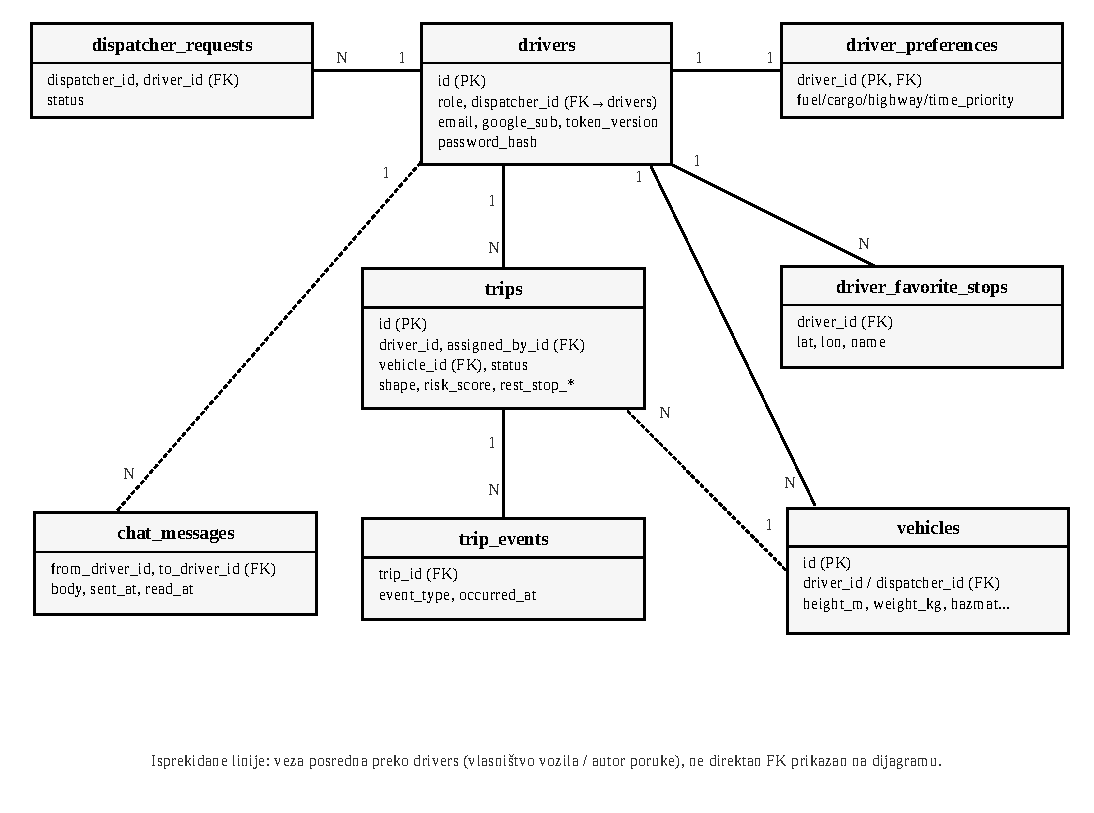
\includegraphics[width=0.88\textwidth]{diagrams/erd.pdf}
\caption{Pregled entiteta baze podataka (skraćeno, bez svih kolona)}
\label{fig:erd}
\end{figure}

Šema baze je organizovana u četiri numerisane, hronološke migracije, upravljane alatom \texttt{goose}, koji garantuje da se svaka migracija primeni tačno jednom, bez obzira na to koliko puta se sistem pokrene. Tabela 7.2 sumira sadržaj svake migracije.

\begin{longtable}{@{}p{0.470\textwidth}p{0.470\textwidth}@{}}
\caption{Migracije šeme baze podataka}\label{tab:7-2}\\
\toprule
\textbf{Migracija} & \textbf{Sadržaj} \\
\midrule
\endhead
\texttt{00001\_initial\_schema.sql} & Osnovna šema: \texttt{drivers}, \texttt{vehicles}, \texttt{trips}, \texttt{driver\_preferences}, \texttt{driver\_favorite\_stops}, \texttt{trip\_events}, \texttt{chat\_messages} \\
\texttt{00002\_dispatcher\_roles.sql} & \texttt{drivers.role}/\texttt{dispatcher\_id}, \texttt{vehicles.dispatcher\_id}, \texttt{trips.assigned\_by\_id}, tabela \texttt{dispatcher\_requests} \\
\texttt{00003\_google\_and\_email\_auth.sql} & \texttt{drivers.google\_sub}/\texttt{email}/\texttt{email\_verified}, tabela \texttt{email\_verification\_tokens} \\
\texttt{00004\_password\_reset\_and\_logout\_all.sql} & \texttt{drivers.token\_version}, tabela \texttt{password\_reset\_tokens} \\
\bottomrule
\end{longtable}

Listing 7.1 prikazuje deo osnovne šeme — tabele \texttt{vehicles} i \texttt{trips}, sa CHECK ograničenjem koje garantuje da osovinsko opterećenje vozila ne može biti veće od njegove ukupne mase (integritetno ograničenje na nivou baze, ne samo na nivou aplikacije).

\begin{lstlisting}[caption={Osnovna šema tabela \texttt{vehicles} i \texttt{trips} (\texttt{00001\_initial\_schema.sql})}]
CREATE TABLE IF NOT EXISTS vehicles (
    id SERIAL PRIMARY KEY,
    height_m DOUBLE PRECISION NOT NULL,
    width_m DOUBLE PRECISION NOT NULL,
    length_m DOUBLE PRECISION NOT NULL,
    weight_kg DOUBLE PRECISION NOT NULL,
    axle_load_kg DOUBLE PRECISION NOT NULL,
    hazmat BOOLEAN NOT NULL DEFAULT false,
    created_at TIMESTAMPTZ NOT NULL DEFAULT now(),
    CHECK (axle_load_kg <= weight_kg)
);

CREATE TABLE IF NOT EXISTS trips (
    id SERIAL PRIMARY KEY,
    vehicle_id INTEGER NOT NULL REFERENCES vehicles(id),
    origin_lat DOUBLE PRECISION NOT NULL,
    origin_lon DOUBLE PRECISION NOT NULL,
    destination_lat DOUBLE PRECISION NOT NULL,
    destination_lon DOUBLE PRECISION NOT NULL,
    distance_km DOUBLE PRECISION NOT NULL,
    duration_min DOUBLE PRECISION NOT NULL,
    risk_score DOUBLE PRECISION NOT NULL,
    shape TEXT NOT NULL,
    status TEXT NOT NULL DEFAULT 'created',
    created_at TIMESTAMPTZ NOT NULL DEFAULT now()
);
\end{lstlisting}

Geometrija rute (\texttt{trips.shape}) čuva se kao enkodovan tekstualni polyline (isti format koji vraća Valhalla), a ne kao PostGIS \texttt{geometry} kolona — pragmatičan izbor koji izbegava dekodiranje/enkodiranje geometrije pri svakom čitanju iz baze, po cenu da prostorni upiti nad geometrijom rute (npr. "sve ture koje prolaze kroz ovaj region") nisu mogući direktno u bazi, već bi zahtevali dekodiranje u aplikacionom sloju — razmatrano kao mogući pravac budućeg rada u poglavlju 10.

\section{Uloge vozač/dispečer}

Sistem razlikuje dve uloge vozača: \textbf{vozač} (\texttt{driver}) i \textbf{dispečer} (\texttt{dispatcher}), zapisane u koloni \texttt{drivers.role}. Veza dispečer↔vozač se, namerno, ne uspostavlja pri registraciji, već isključivo preko mehanizma zahteva i odobrenja: dispečer šalje zahtev (\texttt{POST /dispatcher/requests}) izabranom vozaču, a vozač ga prihvata ili odbija (\texttt{POST /driver/requests/\{id\}/respond}); prihvatanje postavlja \texttt{drivers.dispatcher\_id} na identifikator dispečera. Vozač u svakom trenutku može napustiti dispečera (\texttt{POST /driver/leave-dispatcher}), čime se ta veza raskida.

Vozilo (\texttt{vehicles}) pripada tačno jednom od dva vlasnika — \texttt{driver\_id} ili \texttt{dispatcher\_id} — nikad oboma. Ovim se modeluje realan scenario iz transportne prakse: vozač koji radi za dispečera može voziti vozilo koje je u vlasništvu firme (dispečera), ali isto tako može, paralelno, imati i sopstveno vozilo kojim upravlja samostalno — provera koje vozilo vozač trenutno može koristiti (\texttt{vehicleAccessible}/\texttt{vehicleMutable}) implementirana je na nivou Go handler-a, a ne kao ograničenje baze, jer zavisi i od trenutne dispečer-vozač veze, koja se može promeniti tokom vremena.

Kada dispečer kreira turu za vozača (\texttt{assigned\_by\_id} postavljen na dispečera), ruta se generiše i rangira prema \textbf{dispečerovom} profilu preferenci, ne vozačevom — s obzirom na to da je dispečer taj koji donosi odluku o ruti u ime firme, a preference u ovom sistemu modeluju stil odlučivanja o ruti, ne lične navike vozača u vožnji.

\section{Asinhrona obrada — RabbitMQ i modul pauza vozača}

Kada vozač pokrene turu, backend objavljuje \texttt{trip.started} poruku na \texttt{trip.events} topic exchange RabbitMQ-a. Nezavisan worker proces, pokrenut kao goroutine unutar istog backend binarnog fajla (ne kao poseban kontejner), konzumira tu poruku i računa jednostavan predlog pauze: ako je planirano trajanje ture veće od praga od 270 minuta (4.5h — pojednostavljena zamena za stvarno AETR pravilo o obaveznoj pauzi nakon određenog vremena vožnje \cite{aetr}, obrazloženo dalje u ovom poglavlju), worker pronalazi tačku na ruti gde bi se vozilo teorijski nalazilo nakon isteka tog vremena (pod pretpostavkom konstantne brzine duž rute), i traži najbliže odmaralište iz skupa OSM node-ova učitanih u poglavlju 5.3 koje je stvarno u koridoru trase. Listing 7.2 prikazuje deo implementacije koja računa predlog.

\begin{lstlisting}[caption={Proračun predloga pauze u \texttt{TripWorker} (\texttt{backend/internal/worker/trip\_worker.go})}]
const restThresholdMin = 270 // 4.5h - stand-in za AETR pravilo

func (w *TripWorker) computeRestStop(ctx context.Context, trip store.Trip) store.RestStopSuggestion {
	if trip.DurationMin <= restThresholdMin {
		return store.RestStopSuggestion{}
	}
	afterMin := float64(restThresholdMin)
	suggestion := store.RestStopSuggestion{AfterMinutes: &afterMin}

	points := valhalla.DecodePolyline6(trip.Shape)
	fraction := restThresholdMin / trip.DurationMin
	at := valhalla.PointAtFraction(points, fraction)

	// ... učitavanje preferenci vozača i omiljenih stanica ...
	stop, _, found := w.RestStops.NearestOnRoute(at.Lat, at.Lon, brand, favorites,
		reststop.DefaultPreferredRadiusM, routePoints, reststop.DefaultRouteCorridorRadiusM, hazmat)
	if !found {
		return suggestion
	}
	suggestion.Lat, suggestion.Lon = &stop.Lat, &stop.Lon
	suggestion.Amenity = &stop.Amenity
	return suggestion
}
\end{lstlisting}

Rezultat se upisuje u samu turu (\texttt{trips.rest\_stop\_*} kolone) i u dnevnik događaja (\texttt{trip\_events}, tip \texttt{rest\_stop\_suggested}), koji mobilna aplikacija prikazuje vozaču kao vremensku liniju (poglavlje 8.1). Za vozila koja prevoze opasan teret, pretraga preferira benzinske stanice nad parkinzima (u granicama tolerancije rastojanja), a rezultat u svim slučajevima favorizuje vozačevu omiljenu ili brend-specifičnu stanicu, ako se takva nalazi u koridoru trase.

\textbf{Namerno pojednostavljenje.} Prag od 270 minuta je jednostavna, fiksna zamena za stvarnu evropsku AETR regulativu o radnom vremenu i obaveznim pauzama vozača teretnih vozila \cite{aetr}, koja u stvarnosti razlikuje dnevno i nedeljno vreme vožnje, obavezne dnevne i nedeljne odmore, i dozvoljava određena izuzeća. Puna implementacija te regulative izlazi iz obima ovog rada (obrazloženo u poglavlju 10) — cilj modula je da demonstrira \textbf{mehanizam} (asinhrono računanje predloga na osnovu proteklog vremena vožnje i geografske pretrage najbliže odgovarajuće lokacije), a ne da zameni stvarnu, zakonski obavezujuću logiku.

\textbf{Napomena o evoluciji sistema.} U ranoj fazi razvoja bio je planiran i drugi tok poruka — \texttt{trip.eta\_updated}, koji bi worker objavljivao nakon računanja ETA, a WebSocket gateway (7.5) konzumirao radi guranja ka klijentu. Taj tok je napušten kada je uvedeno praćenje stvarne GPS pozicije vozila (umesto simulacije), pošto je ETA tada postalo jednostavnije računati direktno u WebSocket gateway-u, iz svake nove GPS pozicije (poglavlje 7.5) — čime je \texttt{trip.eta\_updated} poruka postala "mrtav kod" (niko je nije konzumirao) i uklonjena je iz sistema. Ovo je uobičajena i zdrava evolucija u razvoju asinhronog sistema: mehanizam koji je u jednom trenutku bio neophodan postaje suvišan kada se promeni pretpostavka na kojoj je zasnovan, i treba ga ukloniti umesto ostaviti kao neaktivan kod.

\section{Real-time komunikacija — WebSocket gateway}

Paket \texttt{ws} implementira dva WebSocket gateway-a nad istom osnovnom idejom: relej poruka svim zainteresovanim klijentima jedne "teme" (ture ili konverzacije), bez čuvanja stanja konverzacije unutar samog WebSocket sloja.

\textbf{Praćenje pozicije uživo.} Za svaku turu koja je u toku, gateway drži strukturu \texttt{liveTrip} sa skupom pretplatnika (otvorenih WebSocket konekcija) i poslednjom emitovanom pozicijom. Kada vozačev telefon prijavi novu GPS poziciju (\texttt{POST /api/v1/trips/\{id\}/position}), gateway izračunava preostalo rastojanje do odredišta (haversine formula) i procenjeno vreme dolaska na osnovu prosečnog planiranog tempa ture, i tu poruku emituje svim trenutno povezanim pretplatnicima — vozačevom sopstvenom ekranu i, ako postoji, njegovom dispečeru koji istu turu prati na svojoj live mapi (poglavlje 8.2). Novi pretplatnik koji se poveže (ili ponovo poveže) odmah prima poslednju poznatu poziciju, umesto da čeka narednu GPS prijavu — bez ovoga, dispečer koji zatvori i ponovo otvori live mapu ne bi video ništa do naredne GPS prijave vozila, koja može kasniti minutima ako se vozilo ne kreće (GPS prijave se šalju na pomak od određenog broja metara, ne na fiksni interval).

\textbf{Napomena o evoluciji sistema.} Prva verzija ovog gateway-a je, kada još nije stigla nijedna stvarna GPS prijava, simulirala kretanje vozila "hodanjem" duž geometrije rute fiksnim korakom, kao zamenu za stvarni GPS signal tokom razvoja bez pristupa fizičkom vozilu. Kada je testiranje sa stvarnim telefonom postalo dostupno, simulacija je počela da pravi vidljiv "skok" na ekranu u trenutku kada bi stigla prva stvarna GPS prijava (jer se stvarna pozicija po pravilu nije poklapala sa simuliranom) — problem koji je rešen potpunim uklanjanjem simulacije, pošto je do tog trenutka mobilna aplikacija već zahtevala stvaran GPS fix pre nego što dozvoli pokretanje ture (provera blizine polazištu, poglavlje 8.1), čime je simulacija izgubila i svoju originalnu svrhu.

\textbf{Chat.} Chat poruke se, za razliku od pozicije, trajno čuvaju u bazi (\texttt{chat\_messages}) preko REST endpoint-a (\texttt{POST /chats/\{driverId\}/messages}) — REST je "izvor istine" za istoriju razgovora. WebSocket veza (\texttt{GET /ws/chats/\{counterpartId\}}) služi isključivo za isporuku uživo dok je druga strana trenutno povezana: backend objavljuje poslatu poruku na RabbitMQ (\texttt{chat.events} exchange), a WS gateway je samo prosleđuje pretplatniku ako je u tom trenutku povezan — ako nije, poruka je već sačuvana u bazi preko REST poziva i biće učitana pri narednom otvaranju razgovora, bez potrebe za posebnim mehanizmom "neisporučenih" poruka.

\clearpage

\chapter{Mobilna aplikacija}

Mobilna aplikacija je jedinstvena Flutter kodna baza koja se, u zavisnosti od uloge prijavljenog korisnika (poglavlje 7.3), grana na dva različita korisnička toka: vozača i dispečera. Grananje se vrši na jednom mestu (\texttt{entry\_router}), odmah nakon prijave, na osnovu polja \texttt{role} vraćenog sa backend-a.

\section{Tok korisnika — vozač}

Nakon prijave (\texttt{login\_screen}, \texttt{register\_screen} sa izborom uloge vozač/dispečer preko \texttt{SegmentedButton}-a, ili \texttt{forgot\_password\_screen} za obnovu lozinke), samostalni vozač ili vozač koji radi za dispečera dolazi na svoj početni ekran. Ako je trenutno pod dispečerom i čeka na ponuđenu turu, prikazuje mu se \texttt{offered\_trips\_screen} sa ponudama koje treba prihvatiti ili odbiti; u suprotnom, vozač sam pokreće planiranje preko \texttt{route\_request\_screen}.

\textbf{Planiranje rute.} \texttt{route\_request\_screen} omogućava izbor polazišta (trenutna GPS pozicija ili pretraga adrese preko \texttt{address\_search\_field}, koja poziva backend \texttt{GET /geocode} proxy ka Nominatim-u) i odredišta, izbor vozila (preko \texttt{vehicle\_list\_screen}/\texttt{vehicle\_profile\_screen}, gde vozač unosi ili menja visinu, širinu, dužinu, masu, osovinsko opterećenje i prevoz opasnog tereta), i prikaz vraćenih alternativnih ruta na mapi, sortiranih po riziku (poglavlje 6.2), sa mogućim objašnjenjem odstupanja rute (poglavlje 6.3) prikazanim kao tekstualna napomena.

\textbf{Pokretanje i praćenje ture.} Pre pokretanja ture, \texttt{start\_proximity\_status} widget provera da je vozač stvarno u blizini (unutar 500m) prijavljenog polazišta preko GPS-a — namerna provera koja sprečava pokretanje ture "iz kancelarije" i garantuje da je prva pozicija koju backend primi zaista stvaran GPS fix, ne proizvoljna vrednost (relevantno za odluku da se ukloni simulacija pozicije, poglavlje 7.5). Tokom vožnje, \texttt{active\_trip\_screen} prikazuje trenutnu poziciju, procenjeno vreme dolaska i alert za predlog pauze (poglavlje 7.4) primljene preko WebSocket veze (\texttt{trip\_socket.dart}, sa automatskim ponovnim povezivanjem po rastućem intervalu — 1, 2, 5, potom 10 sekundi — u slučaju privremenog prekida konekcije), a \texttt{active\_trip\_banner} ostaje vidljiv i na drugim ekranima aplikacije dok je tura aktivna, kao podsetnik i prečica nazad na \texttt{active\_trip\_screen}. Ako vozač napusti planiranu rutu za više od 300m, backend automatski preračunava novu rutu od trenutne pozicije do istog odredišta (\texttt{POST /trips/\{id\}/reroute}).

\textbf{Dnevnik i istorija.} \texttt{trip\_log\_screen} prikazuje dnevnik događaja jedne ture (\texttt{trip\_events} — polazak, predlog pauze, dolazak) kao vremensku liniju, dok \texttt{trip\_list\_screen} organizuje sve vozačeve ture u tri kategorije (u toku, predstojeće, završene). \texttt{truck\_status\_screen} prikazuje nivo goriva, preostali kilometre do sledećeg servisa i ukupne sate vožnje vozila; \texttt{preferences\_screen} omogućava podešavanje stila vožnje (klizači za prioritet potrošnje goriva, osetljivosti tereta, korišćenja auto-puta i brzine, opisani u poglavlju 6.2) i omiljene benzinske stanice; \texttt{chat\_list\_screen}/\texttt{chat\_thread\_screen} omogućavaju dopisivanje sa dispečerom u realnom vremenu (poglavlje 7.5).

\section{Tok korisnika — dispečer}

Dispečer upravlja flotom vozača i vozila kroz odvojen skup ekrana. \texttt{dispatcher\_home\_screen} je početna tačka; \texttt{dispatcher\_available\_drivers\_screen} prikazuje vozače koji trenutno nisu vezani za nijednog dispečera i omogućava slanje zahteva za povezivanje (poglavlje 7.3), dok \texttt{dispatcher\_requests\_screen} prikazuje status poslatih zahteva. \texttt{dispatcher\_create\_trip\_screen} omogućava kreiranje i dodelu ture jednom od svojih vozača, birajući između vozačevog sopstvenog vozila ili vozila u vlasništvu dispečera (poglavlje 7.3).

Najkompleksniji ekran dispečerskog toka je \texttt{dispatcher\_live\_map\_screen}: prikazuje jednu mapu sa \textbf{N paralelnih WebSocket konekcija}, po jednu za svaku aktivnu turu svojih vozača, i ažurira poziciju svakog vozila na mapi čim gateway (poglavlje 7.5) emituje novu poziciju za odgovarajuću turu. \texttt{dispatcher\_trip\_list\_screen} prikazuje istoriju svih tura koje je dispečer dodelio.

\section{Arhitektura mobilne aplikacije}

Aplikacija je organizovana u standardnu Flutter strukturu: \texttt{screens/} (ekrani navedeni u 8.1/8.2), \texttt{models/} (podatkovne klase koje odgovaraju backend JSON odgovorima — \texttt{driver}, \texttt{vehicle\_profile}, \texttt{trip}, \texttt{trip\_event}, \texttt{route\_result}/\texttt{route\_candidate}, \texttt{chat\_message}, \texttt{dispatcher\_request}, \texttt{driver\_preferences}, \texttt{favorite\_stop}, \texttt{geocode\_result}, \texttt{position\_update}, \texttt{rest\_stop}, \texttt{account\_status}, \texttt{auth\_result}), \texttt{services/} i \texttt{widgets/} (deljene, ponovo iskoristive komponente).

Sloj servisa uključuje: \texttt{api\_client.dart} (centralizovan REST klijent koji, pored slanja zahteva, globalno presreće HTTP 401 odgovor i automatski prebacuje korisnika na ekran za prijavu, umesto da svaki ekran posebno rukuje isticanjem sesije), \texttt{auth\_storage.dart} (lokalno, trajno čuvanje JWT tokena na uređaju), \texttt{chat\_socket.dart} i \texttt{trip\_socket.dart} (WebSocket klijenti sa automatskim ponovnim povezivanjem), \texttt{location\_service.dart} (očitavanje GPS pozicije preko \texttt{geolocator} biblioteke), \texttt{google\_auth.dart} (Google prijava na klijentskoj strani), \texttt{polyline.dart} (dekodiranje enkodovane geometrije rute za prikaz na mapi) i \texttt{route\_observer.dart} (Flutter \texttt{RouteAware} mehanizam koji osvežava podatke na ekranu kada se korisnik na njega vrati nakon zatvaranja nekog drugog ekrana — npr. povratak na listu vozila nakon uređivanja profila vozila).

Među deljenim widgetima ističe se \texttt{radial\_fab\_menu.dart} — radijalni, povlačivi (\emph{draggable}) meni pokrenut iz plutajućeg dugmeta (\emph{floating action button}), korišćen kao glavna navigacija umesto klasične donje trake sa karticama (\emph{bottom navigation bar}), kao i \texttt{email\_verification\_banner} (podsetnik da nalog nije verifikovan) i \texttt{start\_proximity\_status} (opisan u 8.1).

\clearpage

\chapter{Testiranje i evaluacija}

\section{Automatizovano testiranje backend-a}

Backend je testiran automatizovanim, tabelarno-vođenim (\emph{table-driven}) Go testovima, standardnim pristupom u Go ekosistemu gde se više varijacija istog scenarija testira kroz jednu test funkciju sa nizom ulaznih/izlaznih parova. Tabela 9.1 prikazuje broj test funkcija po paketu, na dan pisanja rada; svi navedeni testovi prolaze (\texttt{go test ./...} vraća \texttt{ok} za svaki paket koji sadrži testove).

\setlength{\tabcolsep}{4pt}
\renewcommand{\arraystretch}{1.3}

\begin{longtable}{@{}|>{\small\raggedright\arraybackslash}p{0.26\textwidth}|>{\small\centering\arraybackslash}p{0.11\textwidth}|>{\small\raggedright\arraybackslash}p{0.51\textwidth}|@{}}
\caption{Broj automatizovanih testova po Go paketu}\label{tab:9-1}\\
\hline
\rowcolor{black!12}
\textbf{Paket} & \textbf{Broj testova} & \textbf{Fokus testiranja} \\
\hline
\endhead
\texttt{internal/\allowbreak algorithm} & 15 & Isključivanje nedopustivih ivica/čvorova, poklapanje Dijkstra/A*, penal za skretanje, ponašanje nad realnim OSM podacima \\
\hline
\texttt{internal/scoring} & 6 & Funkcija bodovanja rute, preferenca korisnika, popust za omiljenu stanicu \\
\hline
\texttt{internal/explain} & 8 & Detekcija odstupanja rute, identifikacija vezujuće dimenzije, geometrijska divergencija \\
\hline
\texttt{internal/reststop} & 9 & Pretraga najbližeg odmarališta u koridoru rute, hazmat preferenca, brend/omiljena lokacija \\
\hline
\texttt{internal/auth} & 5 & Izdavanje/parsiranje JWT tokena, provera lozinke, verzija tokena \\
\hline
\texttt{internal/ws} & 4 & Relej pozicije pretplatnicima, replay poslednje pozicije novom pretplatniku \\
\hline
\texttt{internal/httpapi} & 4 & HTTP handleri (integracioni testovi nad REST rutama) \\
\hline
\texttt{internal/geocode} & 6 & Nominatim proxy, throttling \\
\hline
\textbf{Ukupno} & \textbf{57} & \\
\hline
\end{longtable}

\setlength{\tabcolsep}{6pt}

Paket \texttt{internal/algorithm} koristi dve vrste test podataka: (a) male, ručno konstruisane sintetičke grafove (npr. "dijamant" od četiri čvora sa kontrolisanim ograničenjima), pogodne za preciznu proveru jedne izolovane osobine algoritma (npr. "grana sa \texttt{maxheight=3.5} se isključuje za vozilo visine 4.0m"), i (b) stvaran OSM ekstrakt koridora Beograd–Novi Sad (poglavlje 9.2), koji dodatno potvrđuje da implementacija korektno parsira i koristi \emph{stvarne} OSM tagove, ne samo tagove koje je autor sam smislio za potrebe testa.

\section{Evaluacija sopstvenog algoritma nad realnim podacima}

Sopstvena Dijkstra/A* implementacija (poglavlje 6.4) je evaluirana nad stvarnim OSM ekstraktom koridora Beograd–Novi Sad (major-roads-only ekstrakt, \newline \texttt{testdata/beograd-novisad-corridor.osm}), učitanim istim \texttt{LoadOSMXML} mehanizmom koji koristi i produkcioni kod. Ekstrakt se učitava u graf od \textbf{38 265 čvorova i 50 705 usmerenih ivica} — dva reda veličine manje od kompletnog nacionalnog Valhalla grafa (898 337 čvorova, poglavlje 5.2), u skladu sa namerom da ovaj modul bude ograničen, transparentan alat za evaluaciju, ne zamena za Valhallu.

\textbf{Plauzibilnost rute.} Za par tačaka Beograd (44.80, 20.40) – Novi Sad (45.25, 19.85), Dijkstra pretraga (vozilo visine 4.0m, mase 40 000 kg) pronalazi put od \textbf{81,0 km kroz 1899 čvorova}. Za poređenje, Valhalla, nad kompletnim nacionalnim grafom sa punim skupom puteva (ne samo magistralnim), za isti par tačaka vraća rute u rasponu od 84,8 do 92,7 km (u zavisnosti od izabrane alternative), zabeleženo tokom rada na Valhalla integraciji (poglavlje 6.1). Rezultat sopstvenog modula je unutar plauzibilnog opsega — blago kraći, što je i očekivano jer ograničeni ekstrakt sadrži samo magistralne puteve i ne modeluje sve raskrsnice/petlje koje Valhalla uzima u obzir sa kompletnim grafom, a start/cilj pretrage su najbliži čvorovi grafa vazdušnoj liniji do date koordinate, ne tačno iste ulazno-izlazne rampe koje bi Valhalla izabrala.

\textbf{Isključivanje na osnovu stvarnog OSM tag-a.} Nad istim ekstraktom pronađena je stvarna deonica sa tagom \texttt{maxheight=4.3} u centralnoj zoni Beograda. Za vozilo visine 4.0m, Dijkstra pronalazi put od 4036m preko te deonice; za vozilo visine 4.5m (koje premašuje 4,3m ograničenje), pretraga korektno ne pronalazi nijedan put između istih dveju tačaka — u ovom ograničenom, samo-magistralnom ekstraktu ne postoji alternativna deonica koja bi vozilo moglo koristiti umesto isključene, pa je ishod potpuno odsustvo puta, a ne duži zaobilazni put. Ovaj test potvrđuje da mehanizam isključivanja radi korektno na \textbf{stvarnim}, ne samo ručno konstruisanim OSM podacima.

\textbf{Poklapanje Dijkstra i A*\emph{.} Za isti par (Beograd, Novi Sad) i profil, Dijkstra i A*} implementacija vraćaju identičnu cenu puta, što je i teorijski očekivano za dopustivu heuristiku (poglavlje 2.3) — A* ne pronalazi drugačiji (a kamoli lošiji) put, samo ga pronalazi pregledavajući manji broj čvorova. Vremenska analiza (Tabela 9.2) potvrđuje da je pretraga, nad grafom ove veličine, brza u odnosu na jednokratno parsiranje ulaznog XML fajla — 11,3 MB OSM XML-a.

\setlength{\tabcolsep}{4pt}
\renewcommand{\arraystretch}{1.3}

\begin{longtable}{@{}|>{\small\raggedright\arraybackslash}p{0.62\textwidth}|>{\small\centering\arraybackslash}p{0.20\textwidth}|@{}}
\caption{Vreme izvršavanja nad koridorom Beograd–Novi Sad (38 265 čvorova, 50 705 ivica)}\label{tab:9-2}\\
\hline
\rowcolor{black!12}
\textbf{Korak} & \textbf{Vreme} \\
\hline
\endhead
Učitavanje i parsiranje OSM XML ekstrakta (\texttt{LoadOSMXML}) & ≈ 405 ms \\
\hline
Dijkstra pretraga (Beograd → Novi Sad) & ≈ 19,3 ms \\
\hline
A* pretraga (Beograd → Novi Sad) & ≈ 17,1 ms \\
\hline
\end{longtable}

\setlength{\tabcolsep}{6pt}

Rezultat u Tabeli 9.2 potvrđuje očekivanje iz poglavlja 2.3 i 6.4: sama pretraga, jednom kada je graf učitan u memoriju, izvršava se za desetine milisekundi i dominantno je ograničena parsiranjem ulaznih podataka, a ne samim algoritmom pretrage — što je i razlog zbog kojeg je u produkcionom putu ovog sistema izgradnja i održavanje grafa u celosti prepušteno Valhalla-i (poglavlje 5.2, 6.1), koja tu istu vrstu posla radi jednom, unapred, za ceo nacionalni graf, umesto pri svakom zahtevu.

\section{Uticaj prilagođene funkcije rizika — studija slučaja}

Doprinos sopstvenog sloja rangiranja (poglavlje 6.2) u odnosu na "sirov" izbor prve Valhalla alternative ilustrovan je konkretnim slučajem otkrivenim tokom testiranja, na ruti u okolini mesta Radalj. Rana verzija formule bodovanja, koja nije sadržala vremenski član (\texttt{timeTerm}), birala je kao "najbolju" alternativu rutu koja je bila \textbf{47\% duža i 30\% sporija} od druge ponuđene alternative, isključivo zato što je imala povoljniji odnos magistralne i lokalne deonice puta (\texttt{highwayTerm}). Sa stanovišta stvarnog transportnog troška (vreme, gorivo, habanje vozila), taj izbor je bio pogrešan — kraća/brža alternativa je bila objektivno bolji izbor uprkos manje povoljnom \texttt{highwayRatio}.

Dodavanjem \texttt{timeTerm}-a, koji direktno kažnjava kandidata srazmerno njegovom relativnom kašnjenju u odnosu na najbrži kandidat u istom skupu alternativa (poglavlje 6.2, Listing 6.3), formula je počela korektno da favorizuje bržu/kraću rutu u ovom slučaju, bez uklanjanja postojećih članova formule (broj manevara, udeo magistralne deonice, potrošnja, oštri manevri) koji ostaju relevantni u slučajevima kada razlika u trajanju nije toliko izražena. Ovaj slučaj je dobar primer opšte lekcije o dizajnu heurističkih funkcija cene sa više članova: dodavanje novog signala treba motivisati \textbf{konkretnim, uočenim lošim ishodom} postojeće formule, a ne unapred pretpostavljenom kompletnošću — isti princip po kome je i ova formula, i funkcija cene u poglavlju 6.4, iz istog razloga ostala eksplicitno obeležena kao nekalibrisana, prva heuristička procena, a ne konačan, empirijski potvrđen model.

\section{Ograničenja identifikovana testiranjem}

Testiranje je otkrilo i granice sistema koje nisu greške u uobičajenom smislu, već posledice svesno odabranog obima rada:

\begin{itemize}
\item Sopstveni Dijkstra/A* modul (poglavlje 6.4), primenjen na isti par koordinata za koji je poznat slučaj Novi Banovci (poglavlje 6.3), \textbf{ne reprodukuje} taj slučaj — u ograničenom, samo-magistralnom ekstraktu korišćenom za ovaj modul, u okolini Novih Banovaca ne postoji \texttt{maxheight} tag na way nivou. Najverovatnije objašnjenje, dokumentovano tokom razvoja, je da je stvarno ograničenje u tom slučaju zavedeno kao tačkasta (node) prepreka, ne kao way tag, i/ili da geometrijski najkraći put u ograničenom grafu jednostavno ne prolazi kroz tačno tu deonicu koju bi Valhalla, sa svojim potpuno drugačijim, kompletnim grafom i sopstvenom heuristikom, izabrala. Ovo je pošteno prijavljen negativan nalaz, ne prikriven — dodatno naglašava razliku u nameni dva sloja rutiranja u ovom sistemu: Valhalla (sa Explain mehanizmom, poglavlje 6.3) je taj koji stvarno rešava slučaj Novi Banovci u produkciji; sopstveni modul (6.4) demonstrira princip mehanizma isključivanja nad drugim, ali i dalje stvarnim, primerom istog tipa OSM ograničenja (maxheight=4,3 u centralnom Beogradu, poglavlje 9.2).
\item Penal za skretanje u sopstvenoj pretrazi (6.4) je, kako je i dokumentovano u samom kodu, teorijsko pojednostavljenje koje u retkim slučajevima ne garantuje globalno optimalan put po ukupnom penalu za skretanje.
\item Funkcija rizika (6.2) i funkcija cene sopstvene pretrage (6.4) koriste bazne koeficijente koji su prva heuristička procena, ne kalibrisani prema stvarnim podacima o potrošnji goriva, habanju vozila ili statistici saobraćajnih nezgoda — razlika u odnosu na produkcioni sistem bi bila prikupljanje takvih podataka i kalibracija koeficijenata regresijom ili sličnim metodom, što izlazi iz obima ovog rada.
\end{itemize}

\clearpage

\chapter{Zaključak i budući rad}

Ovaj rad je pokazao da se prihvatljivo tačan, transparentan i \textbf{objašnjiv} sistem za rutiranje teretnih vozila može izgraditi nad potpuno otvorenim geografskim podacima (OpenStreetMap) i otvorenim routing engine-om (Valhalla), uz sopstveni algoritamski doprinos koji tim alatima nedostaje. Implementiran je kompletan sistem koji obuhvata: pripremu geografskih podataka specifičnih za teretni saobraćaj (poglavlje 5), backend servis koji generiše, rangira sopstvenom funkcijom rizika i objašnjava predloženu rutu (poglavlje 6 i 7), sopstvenu, nezavisno testiranu Dijkstra/A* implementaciju nad ograničenim, ali stvarnim podacima (poglavlje 6.4, evaluirana u poglavlju 9.2), distribuiranu komunikaciju preko REST API-ja, RabbitMQ posrednika poruka i WebSocket veza (poglavlje 7), i mobilnu aplikaciju za dve različite korisničke uloge — vozača i dispečera (poglavlje 8). Konkretan slučaj (visinsko ograničenje kod Novih Banovaca, poglavlje 6.3) je korišćen kao stvaran, provaljen dokaz da mehanizam objašnjenja rute radi na pravom, a ne samo hipotetičkom problemu, a slučaj Radalj (poglavlje 9.3) kao konkretan primer u kome je sopstvena funkcija rizika ispravila objektivno pogrešan izbor rute.

\section{Doprinosi rada}

Glavni doprinosi rada su:

\begin{enumerate}
\item Sopstveni sloj rangiranja alternativnih ruta prema riziku specifičnom za teretni saobraćaj i preferencama vozača, nad Valhalla alternativama koje engine sam ne rangira (poglavlje 6.2).
\item Automatizovan mehanizam koji vozaču objašnjava zašto predložena ruta odstupa od geometrijski najkraćeg puta, sa geometrijskom (ne pozicionom) detekcijom mesta odstupanja, potvrđen na stvarnom slučaju (poglavlje 6.3).
\item Samostalna, testirana Dijkstra/A* implementacija nad ograničenim podgrafom OSM podataka, sa sopstvenom funkcijom cene i isključivanjem ivica/čvorova na osnovu fizičkih ograničenja vozila, evaluirana nad stvarnim, a ne samo sintetičkim podacima (poglavlje 6.4, 9.2).
\item Kompletan, iako po obimu ograničen, distribuiran sistem — REST API, asinhrona obrada porukama, WebSocket komunikacija u realnom vremenu — sa modelom uloga dispečer/vozač i mehanizmom ponude/prihvatanja ture (poglavlje 7).
\end{enumerate}

\section{Ograničenja rada}

U skladu sa realno postavljenim obimom (obrazloženim već u poglavlju 1.2), rad svesno ne obuhvata:

\begin{itemize}
\item \textbf{Punu AETR regulativu} o radnom vremenu i pauzama vozača (poglavlje 7.4) — trenutni prag od 270 minuta je pojednostavljena zamena, ne zakonski obavezujuća logika.
\item \textbf{Elevacioni (nagibni) rizik rute} — sistem nema pristup podacima o nagibu puta, pa je procena potrošnje goriva (poglavlje 6.2) relativna, ne apsolutna veličina.
\item \textbf{Offline režim rada mobilne aplikacije} — aplikacija zahteva internet konekciju za svaku operaciju; rad bez signala/na lokalnoj mreži nije podržan.
\item \textbf{Podršku za više država} — geografski podaci i pripremljen graf pokrivaju isključivo teritoriju Republike Srbije.
\item \textbf{Produkcioni nivo bezbednosti} — WebSocket \texttt{CheckOrigin} je propustljiv (poglavlje 4.3), a RabbitMQ topologija je minimalna (jedan topic exchange, bez retry/DLQ mehanizma), prihvatljivo za sistem sa jednim poznatim klijentom, ne za javni, višezakupčani servis.
\item \textbf{Kalibraciju koeficijenata funkcije rizika i funkcije cene} prema stvarnim empirijskim podacima (poglavlje 9.4) — koeficijenti su prva heuristička procena.
\item \textbf{Prostorne upite nad geometrijom rute direktno u bazi} — geometrija se čuva kao tekstualni polyline, ne PostGIS \texttt{geometry} kolona (poglavlje 7.2), iako je PostGIS ekstenzija već deo infrastrukture.
\end{itemize}

\section{Pravci budućeg rada}

Na osnovu ograničenja iz 10.2, prirodni pravci budućeg razvoja su: (1) implementacija pune AETR logike, uključujući razliku između dnevnog i nedeljnog vremena vožnje i zakonski propisanih izuzetaka; (2) uvođenje elevacionih podataka (npr. iz SRTM ili sličnog izvora) u funkciju rizika, radi realnije procene potrošnje goriva na deonicama sa izraženim nagibom; (3) offline režim mobilne aplikacije sa lokalnim kešom poslednje poznate rute i odloženim slanjem GPS pozicija po povratku konekcije; (4) proširenje geografskog obuhvata na region ili celu Evropu, što bi zahtevalo i preispitivanje da li ograničeni, u memoriji učitan skup odmarališta (poglavlje 5.3) i dalje skalira, ili treba preći na PostGIS prostorni upit nad već postojećom ekstenzijom; (5) prikupljanje stvarnih podataka (npr. iz simulacije ili pilot upotrebe) radi kalibracije koeficijenata funkcije rizika (6.2) i funkcije cene sopstvenog algoritma (6.4) regresijom ili sličnim metodom, umesto ručno pretpostavljenih vrednosti; (6) bezbednosni hardening WebSocket sloja (stroža \texttt{CheckOrigin} provera, autentifikacija na nivou pojedinačne poruke) i proizvodna RabbitMQ topologija (retry, dead-letter queue) ako bi sistem prešao iz demonstracionog u produkcioni kontekst sa nepoznatim, nepoverljivim klijentima.

\clearpage


% \bibliography{} below prints its own \chapter*{\bibname} heading (see the
% \renewcommand{\bibname}{...} above) - do not also \chapter*{} it here, that
% would produce two headings.
\addcontentsline{toc}{chapter}{Literatura}
\bibliographystyle{ieeetr}
\bibliography{references}

\chapter*{Spisak skraćenica}
\addcontentsline{toc}{chapter}{Spisak skraćenica}
\begin{longtable}{@{}p{0.18\textwidth}p{0.72\textwidth}@{}}
\toprule
\textbf{Skraćenica} & \textbf{Značenje} \\
\midrule
\endhead
AETR & Evropski sporazum o radu posade vozila koja obavljaju međunarodne drumske prevoze (\emph{Accord européen sur les Transports Routiers}) \\
AMQP & \emph{Advanced Message Queuing Protocol} \\
API & \emph{Application Programming Interface} \\
CRUD & \emph{Create, Read, Update, Delete} \\
ETA & \emph{Estimated Time of Arrival} --- procenjeno vreme dolaska \\
GPS & \emph{Global Positioning System} \\
HGV & \emph{Heavy Goods Vehicle} --- teško teretno vozilo \\
HTTP & \emph{Hypertext Transfer Protocol} \\
JSON & \emph{JavaScript Object Notation} \\
JWT & \emph{JSON Web Token} \\
JWKS & \emph{JSON Web Key Set} \\
MVP & \emph{Minimum Viable Product} \\
OSM & \emph{OpenStreetMap} \\
REST & \emph{Representational State Transfer} \\
SMTP & \emph{Simple Mail Transfer Protocol} \\
SQL & \emph{Structured Query Language} \\
VRP & \emph{Vehicle Routing Problem} \\
WS & WebSocket \\
\bottomrule
\end{longtable}

% \listoffigures / \listoftables below print their own \chapter*{...} heading
% (\listfigurename/\listtablename, see main.tex) - no separate \chapter* here.
\addcontentsline{toc}{chapter}{Spisak slika}
\listoffigures

\addcontentsline{toc}{chapter}{Spisak tabela}
\listoftables

\chapter*{Spisak listinga}
\addcontentsline{toc}{chapter}{Spisak listinga}
\lstlistoflistings

\chapter*{Biografija}
\addcontentsline{toc}{chapter}{Biografija}

\Autor{} rođen/a je [DATUM ROĐENJA] godine u [MESTO ROĐENJA]. Osnovne akademske studije na Fakultetu tehničkih nauka Univerziteta u Novom Sadu, studijski program [STUDIJSKI PROGRAM], upisao/la je [GODINA UPISA] godine. Tokom studija se posebno interesovao/la za oblasti [OBLASTI INTERESOVANJA -- npr. distribuirani sistemi, mobilne aplikacije, geografski informacioni sistemi]. Ovaj diplomski rad predstavlja rezultat rada na projektu razvoja sistema za rutiranje teretnih vozila, izrađenog pod mentorstvom \Mentor.

\bigskip
\textit{(Ovaj odeljak popunjava kandidat/kinja ličnim podacima pre predaje rada.)}


\end{document}
